\section{Axiomatisation of Interval Algebras}
\label{sec:axiomatisation}

{\color{orange} QUESTION I think I should keep this definition, but I am unsure where it would
fit best. For now I have left it here, but maybe it would be better in the background section
somewhere at the start?}

\begin{defn}
  We define the language of strict linear orders $\lslo$ as the single binary relation $\{ < \}$.

  We define the theory of strict linear orders as
  \begin{align*}
    \tslo = \{ & \forall a, \lnot\ (a < a), \\
              & \forall a, \forall b, \forall c, (a < b) \land (b < c) \rightarrow (a < c) \\
              & \forall a, \forall b, (a < b) \lor (a = b) \lor (b < a) \}
  \end{align*}
\end{defn}

\begin{defn}
  We define the language of Allen interval algebras $\laia$ as
  \begin{equation*}
    \laia = \{ \before, \meets, \overlaps, \starts, \finishes, \contained,
               \after, \metby, \overlappedby, \startedby, \finishedby, \contains \}
  \end{equation*}
\end{defn}

The theory of Allen interval algebras follows closely with Allen's main concerns. We must specify
that our relation symbols are both exhaustive and mutually exclusive. It is also important that
our dual relation symbols act as such, otherwise the reasoning possible would not match with the
reasoning done by the interval algebra algorithm. Finally, we need to encode the various
transitivity-like requirements, which is another crucial feature of the algorithm we saw.

Let $I = \{<,m,o,s,f,d,>,M,O,S,F,D\}$, so we can express the notion of exhaustability with the sentence
\begin{equation*}
  \defformula{\text{exh}} = \forall I,\;\forall J,\;
    \bigvee_{i \in I} (I \aiaarrow{i} J)
\end{equation*}
% \begin{align*}
%   \defformula{\text{exh}}  & = \forall I,\;\forall J,\;
%     (I \before J) \lor (I \meets J) \lor (I \overlaps J) \lor (I \starts J)
%         \lor (I \finishes J) \lor (I \contained J) \\
%       & \lor (I = J)  (I \after J) \lor (I \metby J) \lor (I \overlappedby J) \lor (I \startedby J)
%         \lor (I \finishedby J) \lor (I \contains J)
% \end{align*}
And the mutual exclusivity requirement by
\begin{equation*}
  \defformula{\text{mutex}} = \forall I,\;\forall J,\;
    \bigwedge_{\shortstack{$i,j \in I$\\$i \neq j$}}
      \lnot \left( (I \aiaarrow{i} J) \land (I \aiaarrow{j} J) \right)
\end{equation*}
The duality is given by the following sentences
\begin{align*}
  \defformula{\text{dual}_>} & = \forall I,\;\forall J,\; (I \before J) \leftrightarrow (J \after I) \\
  \defformula{\text{dual}_m} & = \forall I,\;\forall J,\; (I \meets J) \leftrightarrow (J \metby I) \\
  \defformula{\text{dual}_o} & = \forall I,\;\forall J,\; (I \overlaps J) \leftrightarrow (J \overlappedby I) \\
  \defformula{\text{dual}_s} & = \forall I,\;\forall J,\; (I \starts J) \leftrightarrow (J \startedby I) \\
  \defformula{\text{dual}_f} & = \forall I,\;\forall J,\; (I \finishes J) \leftrightarrow (J \finishedby I) \\
  \defformula{\text{dual}_d} & = \forall I,\;\forall J,\; (I \contained J) \leftrightarrow (J \contains I)
\end{align*}
And finally, the transitivity of the different relations is given by the following schema, where we
range $i,j$ over $I$ and use $T(i,j)$ to denote the entry under row $i$ and column $j$ of
\cref{tab:transitivity}.
\begin{equation*}
  \defformula{\text{trans}_{i,j}} = \forall I,\;\forall J,\;\forall K,\;
    (I \aiaarrow{i} J) \land (J \aiaarrow{j} K) \rightarrow (I \aiaarrow{T(i,j)} J)
\end{equation*}
With this, we can now give the theory of interval algebras

\begin{defn}
  We define the theory of Allen interval algebras $\taia$ as
  \begin{equation*}
    \taia = \{\defformula{\text{exh}}, \defformula{\text{mutex}}, \defformula{\text{dual}_>},
      \defformula{\text{dual}_m}, \defformula{\text{dual}_o}, \defformula{\text{dual}_s},
      \defformula{\text{dual}_f}, \defformula{\text{dual}_d}\}
      \cup \{ \defformula{\text{trans}_{i,j}}\ |\ i,j \in I \}
  \end{equation*}
\end{defn}

% ------ Justifying this axiomatisation of interval algebras

With a theory defined, the first thing to determine is whether or not it is satisfiable, since an
inconsistent theory would not be very interesting. The most natural models we want should come from
non-zero intervals over linear orders, which we now check.

\begin{defn}
  Given a linear order $L$ we define its set of non-zero intervals $\inter[P]$ as the set
  \begin{equation*}
    \inter[L] = \left\{(x_1,x_2)\ |\ x_1 < x_2 \right\} \subseteq L^2
  \end{equation*}
  We can turn this into a $\laia$-structure under the interpretations:
  \begin{itemize}
    \item $(x_1,x_2) \aiaarrow{i} (y_1,y_2)$ if and only if
      $L \models \defformula{\aiaarrow{i}}(x_1,x_2,y_1,y_2)$.
    \item $(x_1,x_2) \raiaarrow{i} (y_1,y_2)$ if and only if
      $L \models \defformula{\aiaarrow{i}}(y_1,y_2,x_1,x_2)$.
  \end{itemize}
  where we range $i$ over the indexing set $\aiaindex$ and define the first order
  $\lslo$-formulas by
  \begin{align*}
    \beforef(x_1,x_2,y_1,y_2)    & = \left(x_1 < x_2\right) \land \left(x_2 < y_1\right) \land
      \left(y_1 < y_2\right) \\
    \meetsf(x_1,x_2,y_1,y_2)     & = \left(x_1 < x_2\right) \land \left(x_2 = y_1\right) \land
      \left(y_1 < y_2\right) \\
    \overlapsf(x_1,x_2,y_1,y_2)  & = \left(x_1 < y_1\right) \land \left(y_1 < x_2\right) \land
      \left(x_2 < y_2\right) \\
    \startsf(x_1,x_2,y_1,y_2)    & = \left(x_1 = y_1\right) \land \left(y_1 < x_2\right) \land
      \left(x_2 < y_2\right) \\
    \finishesf(x_1,x_2,y_1,y_2)  & = \left(y_1 < x_1\right) \land \left(x_1 < x_2\right) \land
      \left(x_2 = y_2\right) \\
    \containedf(x_1,x_2,y_1,y_2) & = \left(y_1 < x_1\right) \land \left(x_1 < x_2\right) \land
      \left(x_2 < y_2\right) \\
  \end{align*}
\end{defn}

Notice that the subset $\inter[L] \subseteq L^2$ is definable using the language of strict linear
orders. Similarly, the interpretations of the relations are also given by formulas in this language.
As a result, the structure $\inter[L]$ is interpretable in the strict linear order $L$.

\begin{thm}
  Given a strict linear order $L$, $\inter[L]$ is a model of $\taia$ under the above
  interpretations.
\end{thm}
\begin{proof}
  First we check that $\inter[L] \models \defformula{\text{exh}}$. We want to count the number of
  possible arrangements of $x_1,x_2,y_1,y_2 \in L$ under the restriction that $x_1 < x_2$ and
  $y_1 < y_2$. Since we need $x_1 < x_2$, we can start with just the following
  \begin{center}
    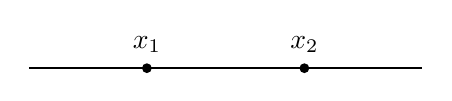
\begin{tikzpicture}
      \draw[thick, -] (0,0) -- (5,0);
      \node[circle,fill,inner sep=1.25pt,label=above:${x_1}$] (1) at (1.5,0) {};
      \node[circle,fill,inner sep=1.25pt,label=above:${x_2}$] (2) at (3.5,0) {};
    \end{tikzpicture}
  \end{center}
  Then there are 5 possible positions for $y_1$: we can have $y_1 = x_i$ for some $i$ or $y_1$ can
  lie on one of the lines, distinct from both $x_1$ and $x_2$. Then, since we need $y_1 < y_2$, the
  number of possible arrangements can be seen to be $5 + 5 + 3 + 3 + 1 = 13$. Including equality,
  we have 13 relation symbols, each representing a different ordering between the $x_i$ and $y_i$,
  which must mean that our relation symbols are exhaustive after all.

  Next we check that the relation symbols are mutually exclusive. This comes from the fact that each
  relation symbol encodes a separate possible ordering between the interval start and end points.
  As it is not possible to have 2 different orderings of the same fixed elements, the relation
  symbols must be mutually exclusive. For example, suppose that we have
  \begin{equation*}
    (x_1,x_2) \before (y_1,y_2) \qquad\qquad
    (x_1,x_2) \overlaps (y_1,y_2)
  \end{equation*}
  This happens only if we have both
  \begin{equation*}
    x_1 < x_2 < y_1 < y_2 \qquad\qquad
    x_1 < y_1 < x_2 < y_2
  \end{equation*}
  and so $x_2 < y_1 < x_2$. Since $<$ is irreflexive, this cannot happen.

  Checking transitivity is quite routine, the main difficulty being the sheer amount of cases. We
  will explicitly check the upper left quadrant in \cref{tab:transitivity} and leave the rest for
  the diligent reader. Fix $(x_1,x_2), (y_1,y_2), (z_1,z_2) \in \inter[L]$, which we will denote by
  $x,y,z$ respectively, then:
  \begin{itemize}
    \item Suppose that $x \before y$, so $x_1 < x_2 < y_1 < y_2$. If
      $y \aiaarrow{<mos} z$ then in all cases we must have
      $y_1 \leq z_1$, hence $x_1 < x_2 < z_1 < z_2$ and $x \before z$. On the other
      hand, if $y \aiaarrow{fd} z$ then we have $z_1 < y_1 \leq z_2$. This means
      that $x_2 < z_2$, restricting the possible relations between $x$ and $z$ to
      $x \aiaarrow{<mosd} z$ as expected.
    \item Suppose that $x \meets y$ so $x_1 < x_2 = y_1 < y_2$. If
      $y \aiaarrow{<mo} z$ then in all cases we must have $y_1 < z_1$ implying that
      $x \before z$. If $y \starts z$ then $y_1 = z_1 < z_2$ and
      $x \meets z$ too. Finally, if $y \aiaarrow{fd} z$ then we have
      $z_1 < y_1 < y_2 \leq z_2$, but $x_2 = y_1$ implying that $x \aiaarrow{osd} z$.
    \item Suppose that $x \overlaps y$, in which case we have $x_1 < y_1 < x_2 < y_2$. Then if
      $y \aiaarrow{<m} z$ we see that $x_1 < x_2 < z_1 < z_2$ so $x \before z$. If $y \overlaps z$
      then $x_1 < z_1$ and $x_2 < z_2$, leaving $x \aiaarrow{<mo} z$ as the only options. If
      $y \starts z$ then $x_1 < y_1 = z_1 < x_2 < y_2 < z_2$ so $x \overlaps z$ too. On the other
      hand if $y \aiaarrow{fd} z$ then $z_1 < x_2 < z_2$ and hence $x \aiaarrow{osd} z$.
    \item Suppose that $x \starts y$ so $x_1 = y_1 < x_2 < y_2$. In the case that $y \aiaarrow{<m} z$
      then $x_1 < x_2 < z_1 < z_2$, ie. $x \before z$. Similarly to before, if $y \overlaps z$ then
      $x_1<z_2$ and $x_2 < z_2$, so $x \aiaarrow{<mo} z$. If $y \starts z$ then we get
      $x_1 = y_1 = z_1 < x_2 < y_2 < z_2$ so $x \starts z$ too. For the last case, if
      $y \aiaarrow{fd} z$ then $z_1 < y_1 = x_1 < x_1 < y_2 \leq z_2$ so $x \contained z$.
    \item Suppose that $x \finishes y$, then $y_1 < x_1 < x_2 = y_2$. If $y \before z$ then we get
      $x_1 < x_2 = y_2 < z_1 < z_2$ and so $x \before z$. If $y \meets z$ then similarly we have
      $x_1 < x_2 = y_2 = z_1 < z_2$ so $x \meets z$.  In the case that $y \overlaps z$ we can see
      that $z_1 < y_2 = x_2 < z_2$ so $x \aiaarrow{osd} z$. If $x \aiaarrow{sd} z$ then
      $z_1 < y_1 = x_1 < x_2 < y_2 \leq z_2$, implying $x \contained z$. Finally, if $y \finishes z$
      then $z_1 < y_1 < x_1 < x_2 = y_2 = z_2$ and $x \finishes z$.
    \item Suppose that $x \contained y$ so $y_1 < x_1 < x_2 < y_2$. If $y \aiaarrow{<m} z$ then
      we have $x_1 < x_1 < y_2 \leq z_1 < z_2$ so $x \before z$. If $y \overlaps z$ then all we can
      say is that $x_2 < z_2$, leaving us with $x \aiaarrow{<mosd} z$. For the final case, if
      $y \aiaarrow{sfd} z$ then we end up with $z_1 \leq y_1 < x_1 < x_2 < y_2 \leq z_2$, so
      $x \contained z$.
  \end{itemize}
  The rest of the cases can be checked similarly.

  Finally, the different duality formulas hold by definition, so
  $\inter[L] \models \taia$.
\end{proof}

\begin{cor}
  Allen's interval algebras are satisfiable
\end{cor}

So the theory is satisfiable and it includes the main class of models we are interested in, models
coming from intervals over linear orders. Since the theory is relational and universal, it also
means that we can pick out any subset of intervals over a linear order and that will also give us a
model of $\taia$, which agrees with our intuition from the work Allen did originally. We will also
see later that every model of $\taia$ can be seen as a substructure of $\inter[L]$ for some linear
order $L$, which bodes well for our axiomatisation. But first, we need to develop some more
machinery.

Consider the function $\peq : \{0,1\}^2 \to \{ \laia-\text{formulas } \phi(I,J)\}$ defined by
\begin{align*}
  \peq(0,0)(I, J) & = (I \starts J) \lor (I \startedby J) \lor (I = J) \\
  \peq(0,1)(I, J) & = (I \metby J) \\
  \peq(1,0)(I, J) & = (I \meets J) \\
  \peq(1,1)(I, J) & = (I \finishes J) \lor (I \finishedby J) \lor (I = J)
\end{align*}
This function takes as inputs tuples $(n,m)$ with $n,m \in \{0,1\}$ and assigns them
the $\laia$-formulas $\peq(n,m)$ with $I$ and $J$ as free variables. We want to use this function
to quotient out the disjoint union $A + A$ in the following way:
\begin{equation*}
  (n,I) \psim (m,J) \iff A \models \peq(n,m)(I,J)
\end{equation*}
Of course, first we need to figure out whether this gives an equivalence relation.

\begin{prop}
  The relation $\psim$ defined as above is an equivalence relation on $A + A$.
\end{prop}
\begin{proof}
  The relation is reflexive, since $\peq(n,n)$ always contains $I = J$ as a disjunct, hence
  $A \models \peq(n,n)(I,I)$ and so $(n,I) \psim (n,I)$.

  The relation is also symmetric, since $A \models \peq(n,m)(I,J)$ if and only if
  $A \models \peq(m,n)(J,I)$. To see this, notice that the formula $\peq(m,n)$ is always given by
  taking the dual of the relation symbols in $\peq(n,m)$. Hence $(n,I) \psim (m,J)$ if and only if
  $(m,J) \psim (n,I)$.

  {\color{orange} TODO prove transitivity}
\end{proof}

\begin{defn}
  Given an Allen interval algebra $A$, we define the points of $A$ as
  \begin{equation*}
    \points[A] = \frac{A + A}{\psim}
  \end{equation*}
\end{defn}

Consider the function $\plt : \{0,1\}^2 \to \{ \laia-\text{formulas } \phi(I,J)\}$ defined by
\begin{align*}
  \plt(0,0)(I,J) & =(I \before J) \lor (I \meets J) \lor (I \overlaps J)
      \lor (I \finishedby J) \lor (I \contains J) \\
  \plt(0,1)(I,J) & = \lnot\,(I \after J) \land \lnot\,(I \metby J) \\
  \plt(1,0)(I,J) & = (I \before J) \\
  \plt(1,1)(I,J) & = (I \before J) \lor (I \meets J) \lor (I \overlaps J)
      \lor (I \starts J) \lor (I \contained J)
\end{align*}
Using this, we may order the start and end points of intervals in $A$, turning $\points[A]$ into
a strict linear order.

\begin{thm}
  Given an Allen interval algebra $A$, the interpretation of the symbol $<$ in $\points[A]$ given by
  $[(n,I)] < [(m,J)] \iff A \models \plt(n,m)(I,J)$ is well-defined and turns $A$ into a model of
  $\tslo$.
\end{thm}
\begin{proof}
  First we must check that this ordering relation on $\points[A]$ is well-defined. For this fix
  intervals $I_1,I_2,J_1,J_2 \in A$ and $n_1,n_2,m_1,m_2 \in \{0,1\}$ and assume that
  \begin{equation*}
    [(n_1,I_1)] = [(n_2,I_2)] < [(m_2,J_2)] = [(m_1,J_1)]
  \end{equation*}
  Then we must show that indeed, $[(n_1,I_1)] < [(m_1,J_1)]$. There are 16 distinct cases which
  we cover in \cref{tab:plt_well_defined}. Since, in each of the cases, with the possible relations
  $I_1 \longrightarrow J_1$ found in the last column, it is definitely the case that
  $A \models \plt(n_1,m_1)(I_1,J_1)$.

  \begin{table}[ht]
    \centering
    \setlength\extrarowheight{5pt}
    \begin{tabular}{|c|c|c|}
      \hline
      $(n_1,n_2,m_1,m_2)$ & Relation between $I_1,I_2,J_1,J_2$ & Relation between $I_1,J_1$ \\
      \hline\hline
      $(0,0,0,0)$ & $I_1 \aiaarrow{s=S} I_2 \aiaarrow{<moFD} J_2 \aiaarrow{s=S} I_1$ &
        $I_1 \aiaarrow{<moFD} J_1$ \\\hline
      $(0,0,0,1)$ & $I_1 \aiaarrow{s=S} I_2 \aiaarrow{<mosfd=OSFD} J_2 \aiaarrow{m} I_1$ &
        $I_1 \aiaarrow{<moFD} J_1$ \\\hline
      $(0,0,1,0)$ & $I_1 \aiaarrow{s=S} I_2 \aiaarrow{<moFD} J_2 \aiaarrow{M} I_1$ &
        $I_1 \aiaarrow{<mosfd=OSFD} J_1$ \\\hline
      $(0,0,1,1)$ & $I_1 \aiaarrow{s=S} I_2 \aiaarrow{<mosfd=OSFD} J_2 \aiaarrow{f=F} I_1$ &
        $I_1 \aiaarrow{<mosfd=OSFD} J_1$ \\\hline
      $(0,1,0,0)$ & $I_1 \aiaarrow{M} I_2 \aiaarrow{<} J_2 \aiaarrow{s=S} I_1$ &
        $I_1 \aiaarrow{<moFD} J_1 $ \\\hline
      $(0,1,0,1)$ & $I_1 \aiaarrow{M} I_2 \aiaarrow{<mosd} J_2 \aiaarrow{m} I_1$ &
        $I_1 \aiaarrow{<moFD} J_1 $ \\\hline
      $(0,1,1,0)$ & $I_1 \aiaarrow{M} I_2 \aiaarrow{<} J_2 \aiaarrow{M} I_1$ &
        $I_1 \aiaarrow{<mosfd=OSFD} J_1$ \\\hline
      $(0,1,1,1)$ & $I_1 \aiaarrow{M} I_2 \aiaarrow{<mosd} J_2 \aiaarrow{f=F} I_1$ &
        $I_1 \aiaarrow{<mosfd=OSFD} J_1$ \\\hline
      $(1,0,0,0)$ & $I_1 \aiaarrow{m} I_2 \aiaarrow{<moFD} J_2 \aiaarrow{s=S} I_1$ &
        $I_1 \aiaarrow{<} J_1$ \\\hline
      $(1,0,0,1)$ & $I_1 \aiaarrow{m} I_2 \aiaarrow{<mosfd=OSFD} J_2 \aiaarrow{m} I_1$ &
        $I_1 \aiaarrow{<} J_1$ \\\hline
      $(1,0,1,0)$ & $I_1 \aiaarrow{m} I_2 \aiaarrow{<moFD} J_2 \aiaarrow{M} I_1$ &
        $I_1 \aiaarrow{<mosd} J_1$ \\\hline
      $(1,0,1,1)$ & $I_1 \aiaarrow{m} I_2 \aiaarrow{<mosfd=OSFD} J_2 \aiaarrow{f=F} I_1$ &
        $I_1 \aiaarrow{<mosd} J_1$ \\\hline
      $(1,1,0,0)$ & $I_1 \aiaarrow{f=F} I_2 \aiaarrow{<} J_2 \aiaarrow{s=S} I_1$ &
        $I_1 \aiaarrow{<} J_1$ \\\hline
      $(1,1,0,1)$ & $I_1 \aiaarrow{f=F} I_2 \aiaarrow{<mosd} J_2 \aiaarrow{m} I_1$ &
        $I_1 \aiaarrow{<} J_1$ \\\hline
      $(1,1,1,0)$ & $I_1 \aiaarrow{f=F} I_2 \aiaarrow{<} J_2 \aiaarrow{M} I_1$ &
        $I_1 \aiaarrow{<mosd} J_1$ \\\hline
      $(1,1,1,1)$ & $I_1 \aiaarrow{f=F} I_2 \aiaarrow{<mosd} J_2 \aiaarrow{f=F} I_1$ &
        $I_1 \aiaarrow{<mosd} J_1$ \\\hline
    \end{tabular}
    \caption{
      All cases to check if the ordering on $\points[A]$ is well defined.
    }
    \label{tab:plt_well_defined}
  \end{table}

  Now we know that our definition of $<$ does not depend on a choice of representative, we need
  to check whether it satisfies $\tslo$:
  \begin{itemize}
    \item \textbf{irreflexivity}: Fix some element $[(n,I)] \in \points[A]$. Since the interval
      algebra relations (along with equality) are mutually exclusive and $I = I$, no other relation
      can hold for the pair $(I,I)$. Regardless of the value of $n$, $\plt(n,n)(I,I)$ does not
      include $I = I$ as a disjunct, so $A \not\models \plt(n,n)(I,I)$ and $<$ is irreflexive.
    \item \textbf{transitivity}: To show transitivity we start by fixing intervals $I,J,K \in A$ and
      assuming that $[(n,I)] < [(m,J)]$ and $[(m,J)] < [(l,K)]$. Then there are 8 cases
      based on the values of $n,m,k \in \{0,1\}$, all of which are considered in
      \cref{tab:plt_trans_000} up to \cref{tab:plt_trans_111}.
    \item \textbf{trichotomy}: Fix two $I,J \in A$. To check the trichotomy condition holds, we need
      to show that for all $n,m \in \{0,1\}$ we have
      \begin{equation*}
        A \models \plt(n,m)(I,J) \lor \peq(n,m)(I,J) \lor \plt(m,n)(J,I)
      \end{equation*}
      There are 3 cases that we must deal with separately to show this:
      \begin{itemize}
        \item First we consider $[(0,I)]$ and $[(0,J)]$. The formula $\plt(0,0)(I,J)$ is a
          disjunction 5 of our basic relations and $\plt(0,0)(J,I)$ the disjunction of its duals.
          Then $\peq(0,0)(I,J)$ is a disjunction of the 2 missing relations and equality. Hence by
          exhaustiveness of the interval algebra relations and equality, it must be the case that
          $A \models \plt(0,0)(I,J) \lor \peq(0,0)(I,J) \lor \plt(0,0)(J,I)$
        \item Next, we consider $[(0,I)]$ and $[(1,J)]$. Notice that the formula $\plt(0,1)(I,J)$
          is the negation of $\peq(0,1)(I,J) \lor \plt(1,0)(J,I)$, hence by the law of the
          excluded middle, the triple disjunction must hold.
        \item Finally we consider $[(1,I)]$ and $[(1,J)]$. The situation here is similar to the
          $n = m = 0$ case, since $\plt(1,1)(I,J)$ is a disjunction of 5 basic relations, then
          $\plt(1,1)(J,I)$ is the disjunction of its duals and $peq(1,1)(I,J)$ is the disjunction
          of the 2 missing relations plus equality.
      \end{itemize}
      When $(n,m)=(1,0)$, since $\psim$ is symmetric, we know that
      \begin{equation*}
        A \models \peq(1,0)(I,J) \iff A \models \peq(0,1)(J,I)
      \end{equation*}
      which allows us to reduce to the second case above.
  \end{itemize}
\end{proof}

In general, this will not be interpretable in the interval algebra $A$, since we need to
take the disjoint union of two sets which is not a priori available in first order logic.
However, provided that $|A| \neq 1$, then it is possible to define quotient $A^2$ by an appropriate
definable equivalence relation, something along the lines of
\begin{equation*}
  \phi(I,J) = \lnot (I = J)
\end{equation*}
So then we would encode $(0,I) \in A + A$ as the pair $(I,I) \in A^2$ and $(1,I) \in A + A$ as
$(I,J) \in A^2$ where $J$ is any interval different from $I$. Modifying the above definitions to
use this encoding would then show that the strict linear order $\inter[A]$ can be interpreted in
$A$.

% {\color{orange} TODO figure out whether or not to keep this.

% Now that this axiomatisation is justified, show that we can't remove any axioms without making
% it into something we do not want.}

% 0 0 0 case
\begin{table}[ht]
  \centering
  \begin{tabular}{| c | c | c || c | c | c || c | c | c |}
    \hline
    $I \to J$ & $J \to K$ & $I \to K$ &
      $I \to J$ & $J \to K$ & $I \to K$ &
      $I \to J$ & $J \to K$ & $I \to K$ \\
    \hline\hline
    \llrow & \olrow & \Dlrow \\
    \lmrow & \omrow & \Dmrow \\
    \lorow & \oorow & \Dorow \\
    \lFrow & \oFrow & \DFrow \\
    \lDrow & \oDrow & \DDrow \\
    \hline
    \mlrow & \Flrow &&&\\
    \mmrow & \Fmrow &&&\\
    \morow & \Forow &&&\\
    \mFrow & \FFrow &&&\\
    \mDrow & \FDrow &&&\\
    \hline
  \end{tabular}
  \caption{
    The transitivity table for the $\istart{I} < \istart{J}$ and $\istart{J} < \istart{K}$ case.
    For this to imply $\istart{I} < \istart{K}$ we need the $I \to K$ columns to all contain a
    subset of the string $<moFD$.
  }
  \label{tab:plt_trans_000}
\end{table}

% 0 0 1 case
\begin{table}[ht]
  \centering
  \begin{tabular}{| c | c | c || c | c | c || c | c | c |}
    \hline
    $I \to J$ & $J \to K$ & $I \to K$ &
      $I \to J$ & $J \to K$ & $I \to K$ &
      $I \to J$ & $J \to K$ & $I \to K$ \\
    \hline\hline
    \llrow & \olrow & \Dlrow \\
    \lmrow & \omrow & \Dmrow \\
    \lorow & \oorow & \Dorow \\
    \lsrow & \osrow & \Dsrow \\
    \lfrow & \ofrow & \Dfrow \\
    \ldrow & \odrow & \Ddrow \\
    \lerow & \oerow & \Derow \\
    \lOrow & \oOrow & \DOrow \\
    \lSrow & \oSrow & \DSrow \\
    \lFrow & \oFrow & \DFrow \\
    \lDrow & \oDrow & \DDrow \\
    \hline
    \mlrow & \Flrow &&&\\
    \mmrow & \Fmrow &&&\\
    \morow & \Forow &&&\\
    \msrow & \Fsrow &&&\\
    \mfrow & \Ffrow &&&\\
    \mdrow & \Fdrow &&&\\
    \merow & \Ferow &&&\\
    \mOrow & \FOrow &&&\\
    \mSrow & \FSrow &&&\\
    \mFrow & \FFrow &&&\\
    \mDrow & \FDrow &&&\\
    \hline
  \end{tabular}
  \caption{
    The transitivity table for the $\istart{I} < \istart{J}$ and $\istart{J} < \iend{K}$ case.
    For this to imply $\istart{I} < \iend{K}$ we need the $I \to K$ columns to all contain a
    subset of the string $<mosfd=OSFD$. Recall that concur is shorthand for $osfd=OSFD$
  }
  \label{tab:plt_trans_001}
\end{table}


% 0 1 0 case
\begin{table}[ht]
  \centering
  \begin{tabular}{| c | c | c |}
    \hline
    $I \to J$ & $J \to K$ & $I \to K$ \\
    \hline\hline
    \llrow \\
    \mlrow \\
    \olrow \\
    \slrow \\
    \flrow \\
    \dlrow \\
    \elrow \\
    \Olrow \\
    \Slrow \\
    \Flrow \\
    \Dlrow \\
    \hline
  \end{tabular}
  \caption{
    The transitivity table for the $\istart{I} < \iend{J}$ and $\iend{J} < \istart{K}$ case.
    For this to imply $\istart{I} < \istart{K}$ we need the $I \to K$ columns to all contain a
    subset of the string $<mofD$.
  }
  \label{tab:plt_trans_010}
\end{table}

% 0 1 1 case
\begin{table}[ht]
  \centering
  \begin{tabular}{| c | c | c || c | c | c || c | c | c |}
    \hline
    $I \to J$ & $J \to K$ & $I \to K$ &
      $I \to J$ & $J \to K$ & $I \to K$ &
      $I \to J$ & $J \to K$ & $I \to K$ \\
    \hline\hline
    \llrow & \flrow & \Slrow \\
    \lmrow & \fmrow & \Smrow \\
    \lorow & \forow & \Sorow \\
    \lsrow & \fsrow & \Ssrow \\
    \ldrow & \fdrow & \Sdrow \\
    \hline
    \mlrow & \dlrow & \Flrow \\
    \mmrow & \dmrow & \Fmrow \\
    \morow & \dorow & \Forow \\
    \msrow & \dsrow & \Fsrow \\
    \mdrow & \ddrow & \Fdrow \\
    \hline
    \olrow & \elrow & \Dlrow \\
    \omrow & \emrow & \Dmrow \\
    \oorow & \eorow & \Dorow \\
    \osrow & \esrow & \Dsrow \\
    \odrow & \edrow & \Ddrow \\
    \hline
    \slrow & \Olrow &&&\\
    \smrow & \Omrow &&&\\
    \sorow & \Oorow &&&\\
    \ssrow & \Osrow &&&\\
    \sdrow & \Odrow &&&\\
    \hline
  \end{tabular}
  \caption{
    The transitivity table for the $\istart{I} < \iend{J}$ and $\iend{J} < \iend{K}$ case.
    For this to imply $\istart{I} < \iend{K}$ we need the $I \to K$ columns to all contain a
    subset of the string $<mosfd=OSFD$. Recall that concur is shorthand for $osfd=OSFD$.
  }
  \label{tab:plt_trans_011}
\end{table}

% 1 0 0 case
\begin{table}[ht]
  \centering
  \begin{tabular}{| c | c | c |}
    \hline
    $I \to J$ & $J \to K$ & $I \to K$ \\
    \hline\hline
    \llrow \\
    \lmrow \\
    \lorow \\
    \lFrow \\
    \lDrow \\
    \hline
  \end{tabular}
  \caption{
    The transitivity table for the $\iend{I} < \istart{J}$ and $\istart{J} < \istart{K}$ case.
    For this to imply $\iend{I} < \istart{K}$ we need the $I \to K$ columns to all contain $<$.
  }
  \label{tab:plt_trans_100}
\end{table}

% 1 0 1 case
\begin{table}[ht]
  \centering
  \begin{tabular}{| c | c | c |}
    \hline
    $I \to J$ & $J \to K$ & $I \to K$ \\
    \hline\hline
    \llrow \\
    \lmrow \\
    \lorow \\
    \lsrow \\
    \lfrow \\
    \ldrow \\
    \lerow \\
    \lOrow \\
    \lSrow \\
    \lFrow \\
    \lDrow \\
    \hline
  \end{tabular}
  \caption{
    The transitivity table for the $\iend{I} < \istart{J}$ and $\istart{J} < \iend{K}$ case.
    For this to imply $\iend{I} < \iend{K}$ we need the $I \to K$ columns to all contain a
    subset of the string $<mosd$.
  }
  \label{tab:plt_trans_101}
\end{table}

% 1 1 0 case
\begin{table}[ht]
  \centering
  \begin{tabular}{| c | c | c |}
    \hline
    $I \to J$ & $J \to K$ & $I \to K$ \\
    \hline\hline
    \llrow \\
    \mlrow \\
    \olrow \\
    \slrow \\
    \dlrow \\
    \hline
  \end{tabular}
  \caption{
    The transitivity table for the $\iend{I} < \iend{J}$ and $\iend{J} < \istart{K}$ case.
    For this to imply $\iend{I} < \istart{K}$ we need the $I \to K$ columns to all contain $<$.
  }
  \label{tab:plt_trans_110}
\end{table}

% 1 1 1 case
\begin{table}[ht]
  \centering
  \begin{tabular}{| c | c | c || c | c | c || c | c | c |}
    \hline
    $I \to J$ & $J \to K$ & $I \to K$ &
      $I \to J$ & $J \to K$ & $I \to K$ &
      $I \to J$ & $J \to K$ & $I \to K$ \\
    \hline\hline
    \llrow & \olrow & \dlrow \\
    \lmrow & \omrow & \dmrow \\
    \lorow & \oorow & \dorow \\
    \lsrow & \osrow & \dsrow \\
    \ldrow & \odrow & \ddrow \\
    \hline
    \mlrow & \slrow &&&\\
    \mmrow & \smrow &&&\\
    \morow & \sorow &&&\\
    \msrow & \ssrow &&&\\
    \mdrow & \sdrow &&&\\
    \hline
  \end{tabular}
  \caption{
    The transitivity table for the $\iend{I} < \iend{J}$ and $\iend{J} < \iend{K}$ case.
    For this to imply $\iend{I} < \iend{K}$ we need the $I \to K$ columns to all contain a
    subset of the string $<mosd$.
  }
  \label{tab:plt_trans_111}
\end{table}

\newpage
\section{A Detour Into Category Theory}
\label{sec:adjunction}

\begin{defn}
  Given a theory $\theory$ over language $\lang$, we denote by $\mods{\lang}{\theory}$ the category
  with objects the models of $\theory$ and arrows the $\lang$-embeddings.
\end{defn}

\begin{rem}
  For brevity, we introduce the notation:
  \begin{equation*}
    \slos := \mods{\lslo}{\tslo} \text{ and } \aias := \mods{\laia}{\taia}
  \end{equation*}
\end{rem}

\begin{thm}
  We can turn $\inter$ into a functor
  \begin{equation*}
    \inter : \slos \to \aias
  \end{equation*}
  by sending arrows $f : M \to N$ in $\slos$ to  $\inter[f] : \inter[M] \to \inter[N]$ defined by
  \begin{equation*}
    \inter[f](x_1, x_2) = (f(x_1), f(x_2))
  \end{equation*}
\end{thm}
\begin{proof}
  First we show that for a $\lslo$-embedding $f : L \to M$ between strict linear orders
  $L,M$, the mapping $\inter[f]$ gives a an $\laia$-embedding. Consider the relations in $\laia$,
  and their interpretations in $\inter[L]$: all of the relations are defined by quantifier-free
  $\lslo$-formulas, whose truth value must be preserved under $\lslo$ embeddings like $f$. Since
  $\inter[f]$ simply applies $f$ pointwise, $\inter[f]$ must preserve the truth value of the
  relation symbols in $\laia$, in other words, it is an $\laia$-embedding.

  Now we just need to check that $\inter$ satisfies the two functor axioms:
  \begin{itemize}
    \item \textbf{preserves identity arrows}: Fix some strict linear order $L$ and some interval
      $(x,y) \in \inter[L]$, then
      \begin{equation*}
        \inter[\id{L}](x,y) = (\id{L}(x), \id{L}(y)) = (x,y)
      \end{equation*}
    \item \textbf{respects arrow composition}: Fix three strict linear orders $L,M,N$ along with
      arrows $f : L \to M$, $g : M \to N$ and some interval $(x,y) \in \inter[L]$, then
      \begin{align*}
        \inter[g \circ f](x,y)
          & = (g \circ f(x), g \circ f(y)) \\
          & = (g(f(x)), g(f(y))) \\
          & = \inter[g](\inter[f](x,y)) \\
          & = \inter[g]\circ\inter[f](x,y)
      \end{align*}
  \end{itemize}
\end{proof}

\begin{thm}
  We can turn $\points$ into a functor
  \begin{equation*}
    \points : \aias \to \slos
  \end{equation*}
  by sending arrows $f : A \to B$ in $\aias$ to $\points[f] : \points[A] \to \points[B]$
  defined by
  \begin{equation*}
    \points[f](0, I) = (0, f(I)) \qquad\text{and}\qquad \points[f](1,I) = (1, f(I))
  \end{equation*}
\end{thm}
\begin{proof}
  Given an arrow $f : A \to B$, we must check that $\points[f]$ is a well defined map, and that it
  is an $\lslo$-embedding. These facts both follow by noticing that $f$ is an
  $\laia$-embedding, so it preserves the truth of quantifier-free $\laia$-formulas, so
  \begin{align*}
    (n,I) \psim (m,J)
      & \iff A \models \peq(n,m)(I,J) \\
      & \iff A \models \peq(n,m)(f(I),f(J)) \\
      & \iff (n,f(I)) \psim (m,f(J))
  \end{align*}
  and similarly
  \begin{align*}
    [(n,I)] < [(m,J)]
      & \iff A \models \plt(n,m)(I,J) \\
      & \iff A \models \plt(n,m)(f(I),f(J)) \\
      & \iff \points[f]([(n,I)]) < \points[f]([(m,J)])
  \end{align*}
  for any two $(n,I),(m,J) \in A + A$, since $\peq(n,m)$ and $\plt(n,m)$ are always quantifier-free.

  Next, to see that $\points$ satisfies the functor axioms:
  \begin{itemize}
    \item \textbf{preserves identity arrows}: Fix some interval algebra $A$ and some element
    $[(n, I)] \in \points[A]$. Then notice that
      \begin{equation*}
        \points[\id{A}]([(n,I)]) = [(n, \id{A}(I))] = [(n,I)] = \id{\points[A]}([(n,I)])
      \end{equation*}
      Hence $\points[\id{A}] = \id{\points[A]}$.
    \item \textbf{respects arrow composition}: Fix interval algebras $A,B,C$ along with arrows
      $f : A \to B$, $g : B \to C$. Then for all elements $[(n,I)] \in \points[A]$:
      \begin{align*}
        \points[g \circ f]([(n,I)])
          & = [(n,g \circ f (I))] \\
          & = [(n, g(f(I)))] \\
          & = \points[g]\left( \points[f]([n,I]) \right) \\
          & = \points[g] \circ \points[f] ([n,I])
      \end{align*}
      Hence $\points[g \circ f] = \points[g] \circ \points[f]$ as expected.
  \end{itemize}
\end{proof}

\begin{rem}
  From now on, given an interval algebra $A$ and interval $I \in A$, we will use
  $\istart{I} := [(0,I)]$ and $\iend{I} := [(1,I)]$ to refer to the respective elements of
  $\points[A]$.
\end{rem}

\begin{thm}
  $\points$ is left adjoint to $\inter$.
\end{thm}
\begin{proof}
  We prove this through the Hom-Set definition of an adjunction, so we wish to find an isomorphism
  $\slos(\points[A],L) \cong \aias(A,\inter[L])$ which is natural in both $A$ and $L$.

  We start by defining the forward map
  \begin{equation*}
    \phi_{A,L} : \slos(\points[A],L) \to \aias(A,\inter[L])
  \end{equation*}
  which sends an $\lslo$-embedding $f : \points[A] \to L$ to the $\laia$-embedding
  \begin{equation*}
    \phi_{A,L}(f) : A \to \inter[L] \quad\text{sending}\quad
      I \mapsto (f(\istart{I}), f(\iend{I}))
  \end{equation*}
  To see this is a $\laia$-embedding, recall that it suffices to consider the $\aiaarrow{i}$
  relations for $i \in \aiaindex$, so we fix two intervals $I,J \in A$ and then:
  \begin{equation*}
    \begin{split}
      I \before J
        & \iff   \iend{I}  <   \istart{J} \\
        & \iff f(\iend{I}) < f(\istart{J}) \\
        & \iff \phi_{A,L}(f)(I) \before \phi_{A,L}(f)(J) \\
      I \meets J
        & \iff   \iend{I}  =   \istart{J} \\
        & \iff f(\iend{I}) = f(\istart{J}) \\
        & \iff \phi_{A,L}(f)(I) \meets \phi_{A,L}(f)(J) \\
      I \overlaps J
        & \iff   \istart{I}  <   \istart{J}  <   \iend{I}  <   \iend{J} \\
        & \iff f(\istart{I}) < f(\istart{J}) < f(\iend{I}) < f(\iend{J}) \\
        & \iff \phi_{A,L}(f)(I) \overlaps \phi_{A,L}(f)(J)
      \end{split}
      \begin{split}
      I \starts J
        & \iff   \istart{I}  =   \istart{J}  <   \iend{I}  <   \iend{J} \\
        & \iff f(\istart{I}) = f(\istart{J}) < f(\iend{I}) < f(\iend{J}) \\
        & \iff \phi_{A,L}(f)(I) \starts \phi_{A,L}(f)(J) \\
      I \finishes J
        & \iff   \istart{J}  <   \istart{I}  <   \iend{I}  =   \iend{J} \\
        & \iff f(\istart{J}) < f(\istart{I}) < f(\iend{I}) = f(\iend{J}) \\
        & \iff \phi_{A,L}(f)(I) \finishes \phi_{A,L}(f)(J) \\
      I \contained J
        & \iff   \istart{J}  <   \istart{I}  <   \iend{I}  <   \iend{J} \\
        & \iff f(\istart{J}) < f(\istart{I}) < f(\iend{I}) < f(\iend{J}) \\
        & \iff \phi_{A,L}(f)(I) \contained \phi_{A,L}(f)(J)
    \end{split}
  \end{equation*}

  Next, we define the inverse map
  \begin{equation*}
    \psi_{A,L} : \aias(A,\inter[L]) \to \slos(\points[A],L)
  \end{equation*}
  which sends an $\laia$-embedding $g : A \to \inter[L]$ to the $\lslo$-embedding given by
  \begin{equation*}
    \psi_{A,L}(f) : \points[A] \to L \quad\text{sending}\quad (n, I) \mapsto
      \left(\letin{(x_0,x_1) := g(I)}{x_n}\right)
  \end{equation*}
  Now, we need to ensure these maps are well defined and that they are indeed $\lslo$-embeddings. To
  check that $\psi_{A,L}(f)$ is well defined, we fix intervals $I,J \in A$ and get three cases to
  consider. In all of these cases we suppose $f(I) = (a,b)$ and $f(J) = (c,d)$:
  \begin{itemize}
    \item If $(0,I) \psim (0,J)$ then we must have
      \begin{equation*}
        A \models (I \starts J) \lor (I \startedby J) \lor (I = J)
      \end{equation*}
      Since $f$ is an $\laia$-embedding, this means that
      \begin{equation*}
        \inter[L] \models (f(I) \starts f(J)) \lor (f(I) \startedby f(J)) \lor (f(I) = f(J))
      \end{equation*}
      Equivalently, the above says that $a = c$, so
      $\psi_{A,L}(f)(\istart{I}) = a = c = \psi_{A,L}(f)(\istart{J})$.
    \item If $(0,I) \psim (1,J)$ then the following is true
      \begin{equation*}
        A \models I \metby J
      \end{equation*}
      Which implies that
      \begin{equation*}
        \inter[L] \models f(I) \metby f(J)
      \end{equation*}
      And this happens exactly when $a = d$, meaning
      $\psi_{A,L}(f)(\istart{I}) = a = d = \psi_{A,L}(f)(\iend{J})$. By symmetry of our equivalence
      relation this also deals with the $(1,I) \psim (0,J)$ case.
    \item If $(1,I) \psim (1,J)$ then
      \begin{equation*}
        A \models (I \finishes J) \lor (I \finishedby J) \lor (I = J)
      \end{equation*}
      And so
      \begin{equation*}
        \points[L] \models (f(I) \finishes f(J)) \lor (f(I) \finishedby f(J)) \lor (f(I) = f(J))
      \end{equation*}
      This implies that $b = d$ so $\psi_{A,L}(f)(\iend{I}) = b = d = \psi_{A,L}(f)(\iend{J})$ as
      needed.
  \end{itemize}

  To show monotonicity of $\psi_{A,L}(f)$ we get 4 distinct cases. Assuming again that
  $f(I) = (a,b)$ and $f(J) = (c,d)$:
  \begin{itemize}
    \item If $\istart{I} < \istart{J}$ then we must have
      \begin{equation*}
        A \models (I \before J) \lor (I \meets J) \lor (I \overlaps J)  \lor (I \finishedby J)
                                \lor (I \contains J)
      \end{equation*}
      Since $f$ is an $\laia$-embedding, this means that
      \begin{align*}
        \inter[L] \models\, & (f(I) \before f(J)) \lor (f(I) \meets f(J)) \lor (f(I) \overlaps f(J)) \\
                            & \qquad \lor (f(I) \finishedby f(J)) \lor (f(I) \contains f(J))
      \end{align*}
      This means the ordering of the elements $a,b,c,d$ must be one of:
      \begin{gather*}
        a < b < c < d \qquad a < b = c = d  \qquad a < c < b < d \\
        a < c < d = b \qquad a < c < d < b
      \end{gather*}
      And in all cases $\psi_{A,L}(f)(\istart{I}) = a < c = \psi_{A,L}(f)(\istart{J})$.
    \item If $\istart{I} < \iend{J}$ then we must have
      \begin{equation*}
        A \models \lnot\,(I \after J) \land \lnot\,(I \metby J)
      \end{equation*}
      Since $f$ is an $\laia$-embedding, this means that
      \begin{equation*}
        \inter[L] \models \lnot\,(f(I) \after f(J)) \land \lnot\,(f(I) \metby f(J))
      \end{equation*}
      This is the case with the most orderings of $a,b,c,d$, having one of:
      \begin{gather*}
        a < b < c < d \qquad a < b = c < d \qquad a < c < b < d \qquad a = c < b < d \\
        c < a < b = d \qquad c < a < b < d \qquad a = c < b = d \qquad c < a < d < b \\
        a = c < d < b \qquad a < c < d = b \qquad a < c < d < b
      \end{gather*}
      In all cases though, $\psi_{A,L}(f)(\istart{I}) = a < d = \psi_{A,L}(f)(\iend{J})$.
    \item If $\iend{I} < \istart{J}$ then we must have
      \begin{equation*}
        A \models I \before J
      \end{equation*}
      Since $f$ is an $\laia$-embedding, this means that
      \begin{equation*}
        \inter[L] \models f(I) \before f(J)
      \end{equation*}
      So in $L$ we must have $a < b < c < d$, and so
      $\psi_{A,L}(f)(\iend{I}) = b < c = \psi_{A,L}(f)(\istart{J})$.
    \item If $\iend{I} < \iend{J}$ then we must have
      \begin{equation*}
        A \models (I \before J) \lor (I \meets J) \lor (I \overlaps J) \lor (I \starts J)
                                \lor (I \contained J)
      \end{equation*}
      Since $f$ is an $\laia$-embedding, this means that
      \begin{align*}
        \inter[L] \models\, & (f(I) \before f(J)) \lor (f(I) \meets f(J)) \lor (f(I) \overlaps f(J)) \\
                          & \qquad \lor (f(I) \starts f(J)) \lor (f(I) \contained f(J)
      \end{align*}
      This gives 5 possible orderings of $a,b,c,d$ in $L$:
      \begin{gather*}
        a < b < c < d \qquad a < b = c = d  \qquad a < c < b < d \\
        a = c < b < d \qquad c < a < b < d
      \end{gather*}
      As $b < d$ in all of these, the ordering is preserved by $\psi_{A,L}(f)$.
  \end{itemize}

  We expect $\phi_{A,L}$ and $\psi_{A,L}$ to be inverses, which is confirmed by the following:
  \begin{itemize}
    \item Pick  any $f : \points[A] \to L$ and $[(n,I)] \in \points[A]$, then
      \begin{align*}
        \psi_{A,L}\left(\phi_{A,L}(f)\right)([(n,I)])
          & = \left( \letin{(x_0,x_1) := \phi_{A,L}(f)(I)}{x_n} \right) \\
          & = \left( \letin{(x_0,x_1) := (f(\istart{I}), f(\iend{I}))}{x_n} \right) \\
          & = f([n, I])
      \end{align*}
    \item Pick any $g : A \to \inter[L]$ and $I \in A$, then
      \begin{equation*}
        \phi_{A,L}\left(\psi_{A,L}(g)\right)(I)
          = \left( \psi_{A,L}(g)(\istart{I}), \psi_{A,L}(g)(\iend{I}) \right)
          = g(I)
      \end{equation*}
  \end{itemize}

  Finally, we just have to check naturality of our isomorphism $\phi_{A,L}$. So pick a
  $\laia$-embedding $f : A \to B$ and a $\lslo$-embeddings $g : L \to M$, we need to show the
  following diagram commutes
  % If modifying diagram, don't forget to add [scale cd=0.99]
  % https://q.uiver.app/?q=WzAsNixbMywwLCJcXHNsb3MoXFxwb2ludHNbQV0sTCkiXSxbMywyLCJcXGFpYXMoQSxcXGludGVyW0xdKSJdLFswLDAsIlxcc2xvcyhcXHBvaW50c1tCXSxMKSJdLFswLDIsIlxcYWlhcyhCLFxcaW50ZXJbTF0pIl0sWzYsMiwiXFxhaWFzKEEsXFxpbnRlcltNXSkiXSxbNiwwLCJcXHNsb3MoXFxwb2ludHNbQV0sTSkiXSxbMiwwLCJcXHNsb3MoXFxwb2ludHNbZl0sTCkiXSxbMywxLCJcXGFpYXMoZixcXGludGVyW0xdKSIsMl0sWzIsMywiXFxwaGlfe0IsTH0iLDJdLFsxLDQsIlxcYWlhcyhBLFxcaW50ZXJbZ10pIiwyXSxbMCw1LCJcXHNsb3MoXFxwb2ludHNbQV0sZykiXSxbNSw0LCJcXHBoaV97QSxNfSJdLFswLDEsIlxccGhpX3tBLEx9IiwyXV0=
  \[\begin{tikzcd}[scale cd=0.99]
    {\slos(\points[B],L)} &&& {\slos(\points[A],L)} &&& {\slos(\points[A],M)} \\
    \\
    {\aias(B,\inter[L])} &&& {\aias(A,\inter[L])} &&& {\aias(A,\inter[M])}
    \arrow["{\slos(\points[f],L)}", from=1-1, to=1-4]
    \arrow["{\aias(f,\inter[L])}"', from=3-1, to=3-4]
    \arrow["{\phi_{B,L}}"', from=1-1, to=3-1]
    \arrow["{\aias(A,\inter[g])}"', from=3-4, to=3-7]
    \arrow["{\slos(\points[A],g)}", from=1-4, to=1-7]
    \arrow["{\phi_{A,M}}", from=1-7, to=3-7]
    \arrow["{\phi_{A,L}}"', from=1-4, to=3-4]
  \end{tikzcd}\]
  We do this by checking both squares individually:
  \begin{itemize}
    \item \textbf{left square}: Pick some $h : \slos(\points[B],L)$ and $I \in A$, then
      \begin{align*}
        \phi_{A,L}(\slos(\points[f],L)(h))(I)
          & = \phi_{A,L}(h \circ \points[f])(I) \\
          & = (h(\points[f](\istart{I})), h(\points[f](\iend{I}))) \\
          & = (h(\istart{f(I)}), h(\iend{f(I)})) \\
          & = \phi_{B,L}(h)(f(I)) \\
          & = \phi_{B,L}(h) \circ f(I) \\
          & = \aias(f,\inter[L])(\phi_{B,L}(h))(I)
      \end{align*}
    \item \textbf{right square}: Pick some $h : \slos(\points[A],L)$ and $I \in A$, then
      \begin{align*}
        \phi_{A,M}(\slos(\points[A],g)(h))(I)
          & = \phi_{A,M}(g \circ h)(I) \\
          & = (g(h(\istart{I})), g(h(\iend{I}))) \\
          & = (g(h(\istart{I})), g(h(\iend{I}))) \\
          & = \inter[g](h(\istart{I}), h(\iend{I})) \\
          & = \inter[g](\phi_{A,L}(h)(I)) \\
          & = \aias(A,\inter[g])(\phi{A,L}(h))(I)
      \end{align*}
  \end{itemize}

  % For an interval algebra $A$ and a strict linear order $L$, we have
  % \begin{equation*}
  %   \text{Hom}(\points[A], L) \cong \text{Hom}(A, \inter[L])
  % \end{equation*}
  % A map of linear orders from the start/end points of A to L, enforces a mapping of interval
  % algebras from A to the intervals of L, by checking where the start/end points of the interval end.

  % The above map is "canonical" so it should be natural in A and L.
\end{proof}

In order to get a bit more familiar with these constructions, it can be beneficial to see why
$\points$ is not right  adjoint to $\inter$, that is, in general
we do not have that
\begin{equation*}
  \aias(\inter[L],A) \cong \slos(L,\points[A])
\end{equation*}
for all strict linear orders $L$
and interval algebras $A$. For example, consider the interval algebra $A$ given by the set
$A = \{I, J, K\}$ with the relations between intervals $I \overlaps J, J \meets K, I \before K$.
Applying the $\points$ construction to $A$ gives a linear order with 5 elements, as can be seen in
\cref{fig:points_example}. We will also need the linear order $L = \{1 < 2 < 3\}$, which
has 3 intervals, as seen in \cref{fig:inter_example}. Now, an order preserving embedding
$f : L \to \points[A]$ simply needs to pick 3 distinct points in $\points[A]$. There are
$\binom{5}{3} = 10$ possible ways of picking 3 distinct points out of $\points[A]$, so we see
that $|\slos(L,\points[A])| = 10$. On the other hand, an embedding of interval algebras
$f : \inter[L] \to A$ must pick out two intervals in $A$ which meet (the images of $(1,2)$ and
$(2,3)$) with the constraint that the "union" of these two intervals exists in $A$. In this specific
case, our only option is that $f((1,2)) = J$ and $f((2,3)) = K$, but there is no interval which
is started by $J$ and finished by $K$, so there is nowhere to map $(1,3)$ to. This means that
$\aias(\inter[L],A) = \emptyset$, so there can be no isomorphism between this and
$\slos(L,\points[A])$.


\begin{figure}[ht]
  \centering
  \begin{tikzpicture}
    \draw[dashed, color=gray, -] (0,0)     -- (0, -3);
    \draw[dashed, color=gray, -] (3,0)     -- (3, -3);
    \draw[dashed, color=gray, -] (2,-0.75) -- (2, -3);
    \draw[dashed, color=gray, -] (6,-0.75) -- (6, -3);
    \draw[dashed, color=gray, -] (10,-1.5) -- (10, -3);

    \draw[thick, |-|] (0,0)     -- (3,0)     node[above, midway] {$I$};
    \draw[thick, |-|] (2,-0.75) -- (6,-0.75) node[above, midway] {$J$};
    \draw[thick, |-|] (6,-1.5)  -- (10,-1.5) node[above, midway] {$K$};

    \draw[thin, -] (0,-3) -- (10,-3);
    \node[circle,fill,inner sep=1.25pt,label=below:$\istart{I}$]            (1) at (0, -3) {};
    \node[circle,fill,inner sep=1.25pt,label=below:$\istart{J}$]            (2) at (2, -3) {};
    \node[circle,fill,inner sep=1.25pt,label=below:$\iend{I}$]              (3) at (3, -3) {};
    \node[circle,fill,inner sep=1.25pt,label=below:{$\iend{J}=\istart{K}$}] (4) at (6, -3) {};
    \node[circle,fill,inner sep=1.25pt,label=below:$\iend{K}$]              (5) at (10, -3) {};

    \node (A)       at (-2, -0.75) {$A$};
    \node (pointsA) at (-2, -3)    {$\points[A]$};
    \draw [very thick,decorate,decoration = {brace}] (-1,-1.6) -- (-1,0.1);
    \draw [very thick,decorate,decoration = {brace}] (-1,-3.3) -- (-1,-2.7);
  \end{tikzpicture}
  \caption{An example of the $\points$ construction.}
  \label{fig:points_example}
\end{figure}

\begin{figure}[ht]
  \centering
  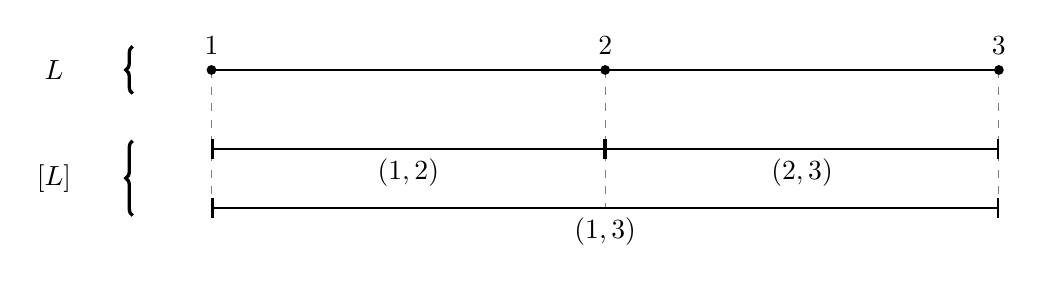
\begin{tikzpicture}
    \draw[dashed, color=gray, -] (0,0) -- (0, -1.75);
    \draw[dashed, color=gray, -] (5,0) -- (5, -1.75);
    \draw[dashed, color=gray, -] (10,0) -- (10, -1.75);

    \draw [thin,-] (0,0) -- (10,0);
    \node[circle,fill,inner sep=1.25pt,label=above:$1$] (1) at (0,0)  {};
    \node[circle,fill,inner sep=1.25pt,label=above:$2$] (2) at (5,0)  {};
    \node[circle,fill,inner sep=1.25pt,label=above:$3$] (3) at (10,0) {};

    \draw[thick, |-|] (0,-1) -- (5,-1) node[below, midway] {$(1,2)$};
    \draw[thick, |-|] (5,-1) -- (10,-1) node[below, midway] {$(2,3)$};
    \draw[thick, |-|] (0,-1.75) -- (10,-1.75) node[below, midway] {$(1,3)$};

    \node (L)      at (-2, 0)     {$L$};
    \node (interL) at (-2, -1.375) {$\inter[L]$};
    \draw [very thick,decorate,decoration = {brace}] (-1,-0.3) -- (-1,0.3);
    \draw [very thick,decorate,decoration = {brace}] (-1,-1.85) -- (-1,-0.9);
  \end{tikzpicture}
  \caption{An example of the $\inter$ construction}
  \label{fig:inter_example}
\end{figure}

Given an adjunction, it is always helpful to compute the associated unit and counit natural
transformations. In our case, the unit is a natural transformation
$\unit{} : \id{\aias} \to \inter[\points]$
whose component at an interval algebra $A$ is given by
$\unit{A} = \phi_{A,\points[A]}(\id{\points[A]})$. Computing this, we get the map
\begin{equation*}
  \unit{A} : A \to \inter[\points[A]] \text{ sending } I \mapsto (\istart{I}, \iend{I})
\end{equation*}
Recall that each component of the unit $\unit{A}$ is an arrow in $\aias$, so it must be an
embedding. This means that every interval algebra $A$ can be seen as a substructure of the intervals
$\inter[L]$ for some appropriate linear order, namely $L = \points[A]$.

Dually, the counit here is a natural transformation $\counit{} : \points[\inter] \to \id{\slos}$
where each of its components is given by $\counit{L} = \psi_{\inter[L],L}(\id{\inter[L]})$.
Fixing some $L$ and working through this construction, we get
\begin{equation*}
  \counit{L} : \points[\inter[L]] \to L \text{ sending }
    \istart{(a,b)} \mapsto a \text{ and } \iend{(a,b)} \mapsto b
\end{equation*}

\begin{prop}
The counit component at a strict linear order $L$, $\counit{L}$, is an isomorphism if and only if
$|L| \neq 1$.
\end{prop}
\begin{proof}
  First, suppose that $|L|=1$, so $L = \{a\}$. Then $\inter[L] = \emptyset$ as we do not allow empty
  intervals and so $\points[\inter[L]] = \emptyset$ too. As such, $\counit{L}$ cannot be an
  isomorphism.

  For the converse, notice that $\counit{L}$ is a map in $\slos$, hence it must be injective.
  Provided that $|L| \neq 1$ then it also turns out to be surjective: fix some
  $a \in L$, there must be at least one distinct $b \in L$. Now either $a < b$, so $(a,b)$ is a
  valid interval over $L$ and then $\counit{L}(\istart{(a,b)}) = a$. Alternatively, $b < a$, so
  $(b, a)$ is an interval in $\inter[L]$ and $\counit{L}(\iend{(b,a)}) = a$
\end{proof}

As for the unit, it will give us an isomorphism when our interval algebra already has all possible
intervals. More precisely, we will say that an interval algebra has all possible intervals if it
satisfies the following sentence
\begin{align*}
  \allints = & \left(\forall I,\; \forall J,\;
        (I \before J)    \rightarrow \exists K,\; (I \meets K)      \land (K \meets J)    \right)\\
    & \land \left(\forall I,\; \forall J,\;
        (I \meets J)     \rightarrow \exists K,\; (I \startedby K)  \land (K \finishes J) \right)\\
    & \land \left(\forall I,\; \forall J,\;
        (I \overlaps J)  \rightarrow \exists K,\; (I \finishedby K) \land (K \starts J)   \right)\\
    & \land \left(\forall I,\; \forall J,\;
        (I \starts J)    \rightarrow \exists K,\; (I \meets K)      \land (K \finishes J) \right)\\
    & \land \left(\forall I,\; \forall J,\;
        (I \finishes J)  \rightarrow \exists K,\; (I \metby K)      \land (K \starts J)   \right)\\
    & \land \left(\forall I,\; \forall J,\;
        (I \contained J) \rightarrow \exists K,\; (I \metby K)      \land (K \starts J)   \right)
\end{align*}

{\color{orange} TODO add something about the uniqueness of such intervals}

\begin{prop}
  The unit component at an interval algebra $A$, $\unit{A}$, is an isomorphism if and only if
  $A \models \allints$.
\end{prop}
\begin{proof}
  First, suppose that $\unit{A}$ is an isomorphism. To show that $A \models allints$ we fix
  two intervals $I,J \in A$. Now we have to consider 6 cases:
  \begin{itemize}
    \item If $I \before J$ then in $\inter[\points[A]]$ we must have
      $\istart{I} < \iend{I} < \istart{J} < \iend{J}$. This means the following are all valid
      intervals
      \begin{equation*}
        \unit{A}(I) = (\istart{I}, \iend{I}) \meets (\iend{I}, \istart{J})
          \meets (\istart{J}, \iend{J}) = \unit{A}(J)
      \end{equation*}
      so taking $K = \unit{A}^{-1}((\iend{I},\istart{J}))$ we see that the first conjunct holds.
    \item If $I \meets J$ then $\istart{I} < \iend{I} = \istart{J} < \iend{J}$, hence taking
      $K = \unit{A}^{-1}((\istart{I}, \iend{J}))$ shows that the second conjunct holds.
    \item If $I \overlaps J$ then $\istart{I} < \istart{J} < \iend{I} < \iend{J}$ and we can take
      $K = \unit{A}^{-1}((\istart{J}, \iend{I}))$ to prove the third conjunct.
    \item If $I \starts J$ then $\istart{I} = \istart{J} < \iend{I} < \iend{J}$, so taking
      $K = \unit{A}^{-1}((\iend{I}, \iend{J}))$ proves the fourth conjunct.
    \item If $I \finishes J$ then $\istart{J} < \istart{I} < \iend{I} = \iend{J}$ so the choice
      $K = \unit{A}^{-1}((\istart{J}, \istart{I}))$ gives a proof of the penultimate conjunct.
    \item If $I \contained J$ then $\istart{J} < \istart{I} < \iend{I} < \iend{J}$ and if we let
      $K = \unit{A}^{-1}((\istart{J}, \istart{I}))$ then we see the last conjunct holds too.
  \end{itemize}
  As all conjuncts hold, this implies that $A \models \allints$ as expected.

  Next, suppose that we have an interval algebra $A$ such that $A \models \allints$ and fix two intervals
  $I,J \in A$. Since $I$ and $J$ are arbitrary, it will suffice to consider the basic non-dual
  relations.
  \begin{itemize}
    \item If $I \before J$ then we get some $K_1$ which is met by $I$ and meets $J$. Then we can glue
      $I$ and $K_1$ to get $K_2$ and similarly we glue $K_1$ and $J$ to get $K_3$. Finally, gluing
      $K_2$ and $J$ gives us $K_4$. This gives the following picture
      \begin{center}
        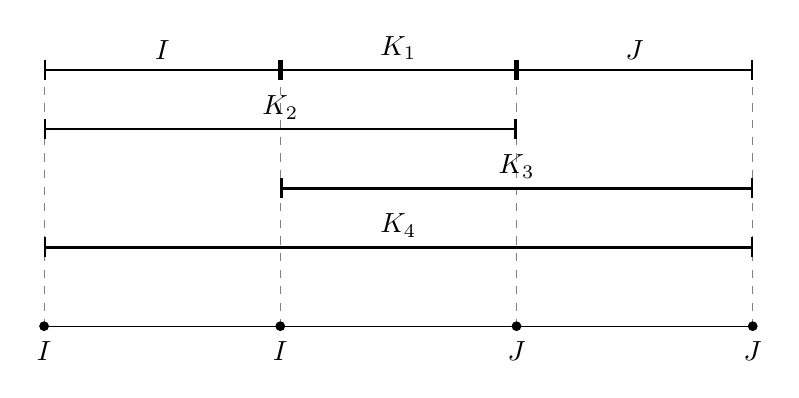
\begin{tikzpicture}
          \draw[dashed, color=gray, -] (0,0) -- (0, -3.25);
          \draw[dashed, color=gray, -] (3,0) -- (3, -3.25);
          \draw[dashed, color=gray, -] (6,0) -- (6, -3.25);
          \draw[dashed, color=gray, -] (9,0) -- (9, -3.25);

          \draw [thin,-] (0,-3.25) -- (9,-3.25);
          \node[circle,fill,inner sep=1.25pt,label=below:$\istart{I}$] (1) at (0,-3.25)  {};
          \node[circle,fill,inner sep=1.25pt,label=below:$\iend{I}$] (2) at (3,-3.25)  {};
          \node[circle,fill,inner sep=1.25pt,label=below:$\istart{J}$] (3) at (6,-3.25) {};
          \node[circle,fill,inner sep=1.25pt,label=below:$\iend{J}$] (3) at (9,-3.25) {};

          \draw[thick, |-|] (0,0) -- (3,0) node[above, midway] {$I$};
          \draw[thick, |-|] (6,0) -- (9,0) node[above, midway] {$J$};
          \draw[thick, |-|] (3,0)  -- (6,0) node[above, midway] {$K_1$};
          \draw[thick, |-|] (0,-0.75)  -- (6,-0.75) node[above, midway] {$K_2$};
          \draw[thick, |-|] (3,-1.5)  -- (9,-1.5) node[above, midway] {$K_3$};
          \draw[thick, |-|] (0,-2.25)  -- (9,-2.25) node[above, midway] {$K_4$};
        \end{tikzpicture}
      \end{center}
      Then the unit $\unit{A}$ surjects on all intervals over the start and end points of $I,J$:
      \begin{align*}
        (\istart{I},\istart{J}) = \unit{A}(K_2) \qquad\qquad (\istart{I},\iend{J}) = \unit{A}(K_4) \\
        (\iend{I},\istart{J}) = \unit{A}(K_1)   \qquad\qquad (\iend{I},\iend{J}) = \unit{A}(K_3)
      \end{align*}
    \item If $I \meets J$ then we can glue $I$ and $J$ to get $K$, yielding the following
      \begin{center}
        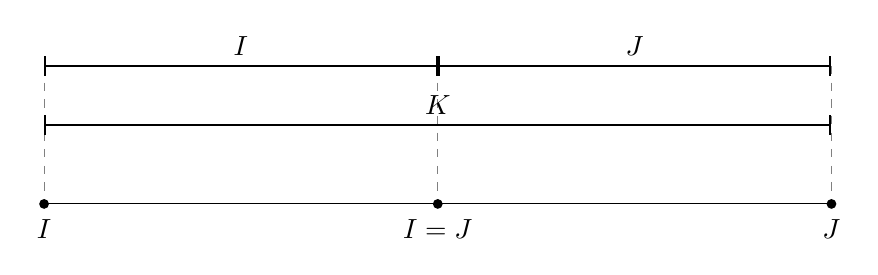
\begin{tikzpicture}
          \draw[dashed, color=gray, -] (0,0) -- (0, -1.75);
          \draw[dashed, color=gray, -] (5,0) -- (5, -1.75);
          \draw[dashed, color=gray, -] (10,0) -- (10, -1.75);

          \draw [thin,-] (0,-1.75) -- (10,-1.75);
          \node[circle,fill,inner sep=1.25pt,label=below:$\istart{I}$] (1) at (0,-1.75)  {};
          \node[circle,fill,inner sep=1.25pt,label=below:${\iend{I}=\istart{J}}$] (2) at (5,-1.75) {};
          \node[circle,fill,inner sep=1.25pt,label=below:$\iend{J}$] (3) at (10,-1.75) {};

          \draw[thick, |-|] (0,0) -- (5,0) node[above, midway] {$I$};
          \draw[thick, |-|] (5,0)  -- (10,0) node[above, midway] {$J$};
          \draw[thick, |-|] (0,-0.75) -- (10,-0.75) node[above, midway] {$K$};
        \end{tikzpicture}
      \end{center}
      The unit also surjects on all valid intervals over the start and end poits of $I,J$:
      \begin{align*}
        (\istart{I},\istart{J}) = \unit{A}(J)   \qquad (\istart{I},\iend{J}) = \unit{A}(K)
          \qquad (\iend{I},\iend{J}) = \unit{A}(J)
      \end{align*}
      In this case there are only 3 in this case since $\iend{I} = \istart{J}$ so
      $(\iend{I}, \istart{J})$ is not a valid interval over $\points[A]$.
    \item If $I \overlaps J$ then first we intersect $I$ and $J$ giving $K_1$. Similarly we can
      intersect $K_1$ with $I$ and $J$ giving $K_2$ and $K_3$ respectively. Finally gluing $I$ and
      $K_3$ together gives $K_4$.
      \begin{center}
        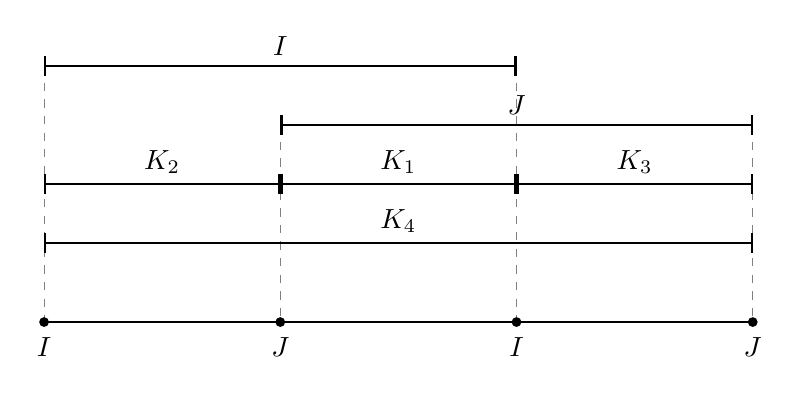
\begin{tikzpicture}
          \draw[dashed, color=gray, -] (0,0) -- (0, -3.25);
          \draw[dashed, color=gray, -] (3,-0.75) -- (3, -3.25);
          \draw[dashed, color=gray, -] (6,0) -- (6, -3.25);
          \draw[dashed, color=gray, -] (9,-0.75) -- (9, -3.25);

          \draw [thin,-] (0,-3.25) -- (9,-3.25);
          \node[circle,fill,inner sep=1.25pt,label=below:$\istart{I}$] (1) at (0,-3.25)  {};
          \node[circle,fill,inner sep=1.25pt,label=below:$\istart{J}$] (2) at (3,-3.25)  {};
          \node[circle,fill,inner sep=1.25pt,label=below:$\iend{I}$] (3) at (6,-3.25) {};
          \node[circle,fill,inner sep=1.25pt,label=below:$\iend{J}$] (3) at (9,-3.25) {};

          \draw[thick, |-|] (0,0) -- (6,0) node[above, midway] {$I$};
          \draw[thick, |-|] (3,-0.75) -- (9,-0.75) node[above, midway] {$J$};
          \draw[thick, |-|] (6,-1.5) -- (9,-1.5) node[above, midway] {$K_3$};
          \draw[thick, |-|] (0,-1.5) -- (3,-1.5) node[above, midway] {$K_2$};
          \draw[thick, |-|] (3,-1.5)  -- (6,-1.5) node[above, midway] {$K_1$};
          \draw[thick, |-|] (0,-2.25)  -- (9,-2.25) node[above, midway] {$K_4$};
        \end{tikzpicture}
      \end{center}
      Similar to the $I \before J$ case, the unit is then surjective onto the 4 possible intervals
      involving $\istart{I}, \iend{I}, \istart{J}, \iend{J}$.
    \item When $I \starts J$ we can intersec $I$ and $J$ to get $K$
      \begin{center}
        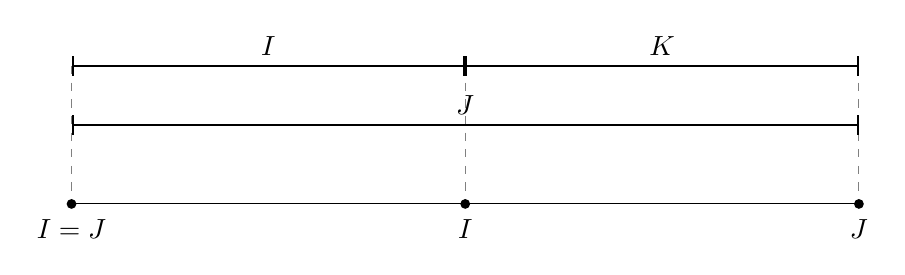
\begin{tikzpicture}
          \draw[dashed, color=gray, -] (0,0) -- (0, -1.75);
          \draw[dashed, color=gray, -] (5,0) -- (5, -1.75);
          \draw[dashed, color=gray, -] (10,0) -- (10, -1.75);

          \draw [thin,-] (0,-1.75) -- (10,-1.75);
          \node[circle,fill,inner sep=1.25pt,label=below:${\istart{I}=\istart{J}}$] (1) at (0,-1.75)  {};
          \node[circle,fill,inner sep=1.25pt,label=below:$\iend{I}$] (2) at (5,-1.75) {};
          \node[circle,fill,inner sep=1.25pt,label=below:$\iend{J}$] (3) at (10,-1.75) {};

          \draw[thick, |-|] (0,0) -- (5,0) node[above, midway] {$I$};
          \draw[thick, |-|] (0,-0.75) -- (10,-0.75) node[above, midway] {$J$};
          \draw[thick, |-|] (5,0)  -- (10,0) node[above, midway] {$K$};
        \end{tikzpicture}
      \end{center}
      We get 4 intervals over the start and end points of $I$ and $J$, which are given by
      \begin{align*}
        (\istart{I},\iend{J}) = \unit{A}(J) \qquad (\istart{I},\iend{I}) = \unit{A}(I)
          \qquad (\iend{I},\iend{J}) = \unit{A}(K)
      \end{align*}
    \item The $I \finishes J$ follows similarly to the previous case, by intersecting $I$ and $J$ to
      get $K$
      \begin{center}
        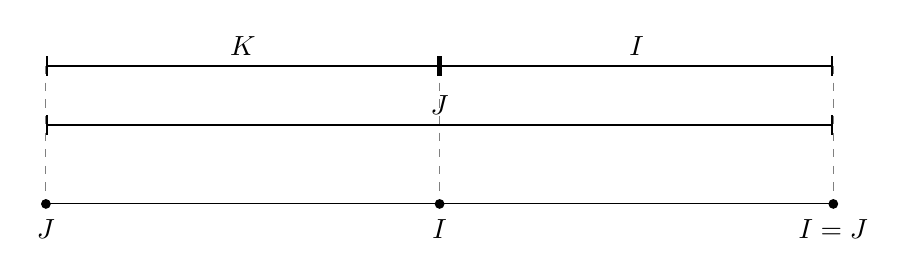
\begin{tikzpicture}
          \draw[dashed, color=gray, -] (0,0) -- (0, -1.75);
          \draw[dashed, color=gray, -] (5,0) -- (5, -1.75);
          \draw[dashed, color=gray, -] (10,0) -- (10, -1.75);

          \draw [thin,-] (0,-1.75) -- (10,-1.75);
          \node[circle,fill,inner sep=1.25pt,label=below:$\istart{J}$] (1) at (0,-1.75)  {};
          \node[circle,fill,inner sep=1.25pt,label=below:$\istart{I}$] (2) at (5,-1.75) {};
          \node[circle,fill,inner sep=1.25pt,label=below:${\iend{I} = \iend{J}}$] (3) at (10,-1.75) {};

          \draw[thick, |-|] (5,0)  -- (10,0) node[above, midway] {$I$};
          \draw[thick, |-|] (0,-0.75) -- (10,-0.75) node[above, midway] {$J$};
          \draw[thick, |-|] (0,0) -- (5,0) node[above, midway] {$K$};
        \end{tikzpicture}
      \end{center}
      And again the 3 valid intervals over $\istart{I},\iend{I},\istart{J},\iend{J}$ all
      lie in the image of the unit
      \begin{align*}
        (\istart{J},\istart{I}) = \unit{A}(K) \qquad (\istart{J},\iend{I}) = \unit{A}(J)
          \qquad (\istart{I},\iend{J}) = \unit{A}(I)
      \end{align*}
    \item Finally there is the $I \contained J$ case. By $\allints$ we can get the initial segment
      $K_1$ of $J$ which meets $I$. Then we intersect $K_1$ and $J$ to get $K_2$, which in turn we
      intersect with $I$ to get $K_3$. Finally gluing $K_1$ and $I$ gives $K_4$.
      \begin{center}
        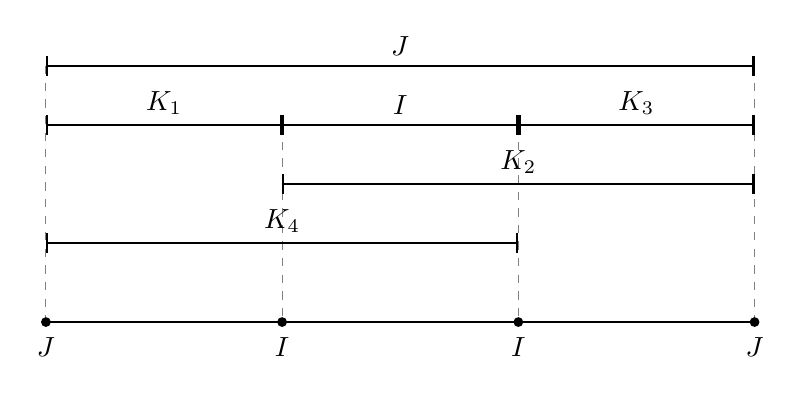
\begin{tikzpicture}
          \draw[dashed, color=gray, -] (0,0) -- (0, -3.25);
          \draw[dashed, color=gray, -] (3,-0.75) -- (3, -3.25);
          \draw[dashed, color=gray, -] (6,-0.75) -- (6, -3.25);
          \draw[dashed, color=gray, -] (9,0) -- (9, -3.25);

          \draw [thin,-] (0,-3.25) -- (9,-3.25);
          \node[circle,fill,inner sep=1.25pt,label=below:$\istart{J}$] (1) at (0,-3.25)  {};
          \node[circle,fill,inner sep=1.25pt,label=below:$\istart{I}$] (2) at (3,-3.25)  {};
          \node[circle,fill,inner sep=1.25pt,label=below:$\iend{I}$] (3) at (6,-3.25) {};
          \node[circle,fill,inner sep=1.25pt,label=below:$\iend{J}$] (3) at (9,-3.25) {};

          \draw[thick, |-|] (0,0) -- (9,0) node[above, midway] {$J$};
          \draw[thick, |-|] (3,-0.75) -- (6,-0.75) node[above, midway] {$I$};
          \draw[thick, |-|] (0,-0.75) -- (3,-0.75) node[above, midway] {$K_1$};
          \draw[thick, |-|] (6,-0.75) -- (9,-0.75) node[above, midway] {$K_3$};
          \draw[thick, |-|] (3,-1.5)  -- (9,-1.5) node[above, midway] {$K_2$};
          \draw[thick, |-|] (0,-2.25)  -- (6,-2.25) node[above, midway] {$K_4$};
        \end{tikzpicture}
      \end{center}
      This gives 4 intervals which all lie in the image of the unit
      \begin{align*}
        (\istart{J},\istart{I}) = \unit{A}(K_1) \qquad\qquad (\istart{J},\iend{I}) = \unit{A}(K_4) \\
        (\istart{I},\iend{J}) = \unit{A}(K_2)   \qquad\qquad (\iend{I},\iend{J}) = \unit{A}(K_3)
      \end{align*}
  \end{itemize}
  This is sufficient to see that $\unit{A}$ is surjective. After all fix some arbitrary interval
  \begin{equation*}
    ([(n,I)], [(m,J)]) \in \inter[\points[A]]
  \end{equation*}
  If $I = J$ then we must have
  \begin{equation*}
    ([(n,I)], [(m,J)]) = (\istart{I}, \iend{I}) = \unit{A}(I)
  \end{equation*}
  If $I \neq J$, then after possibly swapping $I,J$ we may assume $I \aiaarrow{<mosfd}$, which
  brings us to one of the cases handled above, where all intervals involing $\istart{I}, \iend{I},
  \istart{J}$ and $\iend{J}$ were in the image of the unit.
\end{proof}


\begin{cor}
  There exists an equivalence of categories between the full subcategory of strict linear orders $L$
  with $|L| \neq 1$ and the full subcategory of interval algebras satisfying $\allints$.
\end{cor}
\begin{proof}
  An adjunction can always be restricted to an equivalence of categories by considering the full
  subcategories where the unit and counit are isomorphisms.
\end{proof}

% {\color{blue} TODO: consider what our functors do to elementary embeddings?}

\newpage
\section{The Model Theory of Interval Algebras}
\label{sec:model_theory}

\subsection{Fraïssé Class of Finite Interval Algebras}

We start by considering the class $\finaia$ of finite interval algebras. From our work in
\cref{ssub:homogeneous_structures_and_fraisse_classes}, we know that $\finaia$ satisfies the HP,
since $\taia$ is universal and relational. $\laia$ is also finite, so $\finaia$ must be EC.

To prove that $\finaia$ has the JEP and AP, notice that $\points$ must send finite interval algebras
to finite strict linear orders. In fact, given an interval algebra $A$, $|\points[A]| \leq 2|A|$
since $\points[A]$ is a quotient of $A + A$. Similarly, $\inter$ must also send finite strict linear
orders to finite interval algebras as given a strict linear order $L$,
$|\inter[L]| = \binom{|L|}{2}$. Using this fact, we will be able to reduce the proof of these
properties to the proof that $\finslo$ satisfies them.

\begin{prop}
  The class $\finaia$ has the joint embedding property.
\end{prop}
\begin{proof}
  Given two finite interval algebras $A$ and $B$, we use the JEP of strict
  linear orders to get the following diagram in $\slos$
  \[\begin{tikzcd}
    {\points[A]} \\
    && \Omega \\
    {\points[B]}
    \arrow["f", from=1-1, to=2-3]
    \arrow["g"', from=3-1, to=2-3]
  \end{tikzcd}\]
  Then, applying $\inter$ and using the adjunction unit $\eta$, we get
  % https://q.uiver.app/?q=WzAsNSxbMiwwLCJcXGludGVyW1xccG9pbnRzW0FdXSJdLFsyLDIsIlxcaW50ZXJbXFxwb2ludHNbQl1dIl0sWzQsMSwiXFxpbnRlcltcXE9tZWdhXSJdLFswLDAsIkEiXSxbMCwyLCJCIl0sWzAsMiwiXFxpbnRlcltmXSIsMCx7ImNvbG91ciI6WzAsNjAsNjBdfSxbMCw2MCw2MCwxXV0sWzEsMiwiXFxpbnRlcltnXSIsMix7ImNvbG91ciI6WzAsNjAsNjBdfSxbMCw2MCw2MCwxXV0sWzQsMSwiXFx1bml0e0J9IiwyXSxbMywwLCJcXHVuaXR7QX0iXV0=
  \[\begin{tikzcd}
    A && {\inter[\points[A]]} \\
    &&&& {\inter[\Omega]} \\
    B && {\inter[\points[B]]}
    \arrow["{\inter[f]}", color={rgb,255:red,214;green,92;blue,92}, from=1-3, to=2-5]
    \arrow["{\inter[g]}"', color={rgb,255:red,214;green,92;blue,92}, from=3-3, to=2-5]
    \arrow["{\unit{B}}"', from=3-1, to=3-3]
    \arrow["{\unit{A}}", from=1-1, to=1-3]
  \end{tikzcd}\]
  And the composites $\inter[f] \circ \unit{A}$ and $\inter[g] \circ \unit{B}$ along with
  the interval algebra $\Omega$ give us the joint embedding of $A$ and $B$.
\end{proof}

\begin{prop}
  The class $\finaia$ has the amalgamation property.
\end{prop}
\begin{proof}
  Suppose we have the following diagram in $\aias$
  % https://q.uiver.app/?q=WzAsNCxbMiwwLCJBIl0sWzIsMiwiQiJdLFswLDEsIkMiXSxbNCwxXSxbMiwwLCJmIl0sWzIsMSwiZyIsMl1d
  \[\begin{tikzcd}
    && A \\
    C &&&& {} \\
    && B
    \arrow["f", from=2-1, to=1-3]
    \arrow["g"', from=2-1, to=3-3]
  \end{tikzcd}\]
  Applying $\points$ takes us to $\slos$, at which point we can use the AP of strict linear
  orders to get the commuting square
  % https://q.uiver.app/?q=WzAsNCxbMiwwLCJcXHBvaW50c1tBXSJdLFsyLDIsIlxccG9pbnRzW0JdIl0sWzAsMSwiXFxwb2ludHNbQ10iXSxbNCwxLCJcXE9tZWdhIl0sWzIsMCwiXFxwb2ludHNbZl0iLDAseyJjb2xvdXIiOlswLDYwLDYwXX0sWzAsNjAsNjAsMV1dLFsyLDEsIlxccG9pbnRzW2ddIiwyLHsiY29sb3VyIjpbMCw2MCw2MF19LFswLDYwLDYwLDFdXSxbMCwzLCJmJyJdLFsxLDMsImcnIiwyXV0=
  \[\begin{tikzcd}
    && {\points[A]} \\
    {\points[C]} &&&& \Omega \\
    && {\points[B]}
    \arrow["{\points[f]}", color={rgb,255:red,214;green,92;blue,92}, from=2-1, to=1-3]
    \arrow["{\points[g]}"', color={rgb,255:red,214;green,92;blue,92}, from=2-1, to=3-3]
    \arrow["{f'}", from=1-3, to=2-5]
    \arrow["{g'}"', from=3-3, to=2-5]
  \end{tikzcd}\]
  Now going back to $\aias$ gives the commuting diagram
  % https://q.uiver.app/?q=WzAsOSxbNCwwLCJcXGludGVyW1xccG9pbnRzW0FdXSJdLFs0LDIsIlxcaW50ZXJbXFxwb2ludHNbQl1dIl0sWzIsMSwiXFxpbnRlcltcXHBvaW50c1tDXV0iXSxbNiwxLCJcXGludGVyW1xcT21lZ2FdIl0sWzAsMSwiQyJdLFswLDBdLFsxLDBdLFsyLDAsIkEiXSxbMiwyLCJCIl0sWzIsMCwiXFxpbnRlcltcXHBvaW50c1tmXV0iLDEseyJjb2xvdXIiOlswLDYwLDYwXX0sWzAsNjAsNjAsMV1dLFsyLDEsIlxcaW50ZXJbXFxwb2ludHNbZ11dIiwxLHsiY29sb3VyIjpbMCw2MCw2MF19LFswLDYwLDYwLDFdXSxbMCwzLCJcXGludGVyW2YnXSIsMCx7ImNvbG91ciI6WzAsNjAsNjBdfSxbMCw2MCw2MCwxXV0sWzEsMywiXFxpbnRlcltnJ10iLDIseyJjb2xvdXIiOlswLDYwLDYwXX0sWzAsNjAsNjAsMV1dLFs4LDEsIlxcdW5pdHtCfSIsMl0sWzcsMCwiXFx1bml0e0F9Il0sWzQsMiwiXFx1bml0e0N9IiwxXSxbNCw3LCJmIl0sWzQsOCwiZyIsMl1d
  \[\begin{tikzcd}
    {} & {} & A && {\inter[\points[A]]} \\
    C && {\inter[\points[C]]} &&&& {\inter[\Omega]} \\
    && B && {\inter[\points[B]]}
    \arrow["{\inter[\points[f]]}"{description}, color={rgb,255:red,214;green,92;blue,92}, from=2-3, to=1-5]
    \arrow["{\inter[\points[g]]}"{description}, color={rgb,255:red,214;green,92;blue,92}, from=2-3, to=3-5]
    \arrow["{\inter[f']}", color={rgb,255:red,214;green,92;blue,92}, from=1-5, to=2-7]
    \arrow["{\inter[g']}"', color={rgb,255:red,214;green,92;blue,92}, from=3-5, to=2-7]
    \arrow["{\unit{B}}"', from=3-3, to=3-5]
    \arrow["{\unit{A}}", from=1-3, to=1-5]
    \arrow["{\unit{C}}"{description}, from=2-1, to=2-3]
    \arrow["f", from=2-1, to=1-3]
    \arrow["g"', from=2-1, to=3-3]
  \end{tikzcd}\]
  For the AP of the finite interval algebras, we are only interested in the outer square. The
  necessary maps are then $\inter[f'] \circ \unit{A}$ and $\inter[g'] \circ \unit{B}$, both
  mapping into $\inter[\Omega]$.
\end{proof}

\begin{thm}
  The Fraïssé limit of $\finaia$ is $\inter[\Q]$
\end{thm}
\begin{proof}
  To show that the Fraïssé limit of the finite interval algebras is $\inter[\Q]$, it suffices to
  show that $\age(\inter[\Q]) = \finaia$ and that $\inter[\Q]$ is homogeneous.

  To see that $\age(\inter[\Q]) = \finaia$, prove that both sides include into the other.
  Suppose we have some finitely generated $\laia$-substructure $A \subset \inter[\Q]$. Since
  $\taia$ is universal, $A$ must also be an interval algebra. Furthermore, since $\laia$ is
  relational, $A$ must also be finite, so $A \in \finaia$. For the converse inclusion, consider
  some finite interval algebra $A$, it must embed into $\inter[\points[A]]$, which in turn
  embeds into $\inter[\Q]$ (since $\points[A]$ is finite, hence embeddable into $\Q$).
  Restricting these composition of these embeddings onto their image in $\inter[\Q]$ then gives
  the needed isomorphism.

  As for why $\inter[\Q]$ is homogeneous, fix two $\laia$-substructures $A,B \subseteq \inter[\Q]$,
  along with some $\laia$-isomorphism $f : A \to B$. In essence we have the following
  diagram of interval algebras, where $i$ and $j$ are the inclusions into $\inter[\Q]$:
  % https://q.uiver.app/?q=WzAsNCxbMCwyLCJBIl0sWzIsMiwiQiJdLFswLDAsIlxcaW50ZXJbXFxRXSJdLFsyLDAsIlxcaW50ZXJbXFxRXSJdLFswLDEsImYiXSxbMCwyLCJpIl0sWzEsMywiaiIsMl1d
  \[\begin{tikzcd}
    {\inter[\Q]} && {\inter[\Q]} \\
    \\
    A && B
    \arrow["f", from=3-1, to=3-3]
    \arrow["i", from=3-1, to=1-1]
    \arrow["j"', from=3-3, to=1-3]
  \end{tikzcd}\]
  Applying $\inter$ to move to linear orders, we can postcompose $\points[i]$ and $\points[j]$ with
  the counit at $\Q$ to realise $\points[A]$ and $\points[B]$ as $\lslo$-substructures of $\Q$.
  Now, $\points[f]$ is still an isomorphism as these are preserved by functors, and using the
  fact that $\Q$ is homogeneous, we can extend $\points[f]$ to an isomorphism $g$, giving the
  commuting diagram
  % https://q.uiver.app/?q=WzAsNyxbMCw0LCJcXHBvaW50c1tBXSJdLFsyLDQsIlxccG9pbnRzW0JdIl0sWzAsMiwiXFxwb2ludHNbXFxpbnRlcltcXFFdXSJdLFsyLDIsIlxccG9pbnRzW1xcaW50ZXJbXFxRXV0iXSxbMCwwLCJcXFEiXSxbMiwwLCJcXFEiXSxbMCwxXSxbMCwxLCJcXHBvaW50c1tmXSIsMCx7ImNvbG91ciI6WzAsNjAsNjBdfSxbMCw2MCw2MCwxXV0sWzAsMiwiXFxwb2ludHNbaV0iLDAseyJjb2xvdXIiOlswLDYwLDYwXX0sWzAsNjAsNjAsMV1dLFsyLDQsIlxcY291bml0e1xcUX0iXSxbMyw1LCJcXGNvdW5pdHtcXFF9IiwyXSxbMSwzLCJcXHBvaW50c1tqXSIsMix7ImNvbG91ciI6WzAsNjAsNjBdfSxbMCw2MCw2MCwxXV0sWzQsNSwiZyJdXQ==
  \[\begin{tikzcd}
    \Q && \Q \\
    {} \\
    {\points[\inter[\Q]]} && {\points[\inter[\Q]]} \\
    \\
    {\points[A]} && {\points[B]}
    \arrow["{\points[f]}", color={rgb,255:red,214;green,92;blue,92}, from=5-1, to=5-3]
    \arrow["{\points[i]}", color={rgb,255:red,214;green,92;blue,92}, from=5-1, to=3-1]
    \arrow["{\counit{\Q}}", from=3-1, to=1-1]
    \arrow["{\counit{\Q}}"', from=3-3, to=1-3]
    \arrow["{\points[j]}"', color={rgb,255:red,214;green,92;blue,92}, from=5-3, to=3-3]
    \arrow["g", from=1-1, to=1-3]
  \end{tikzcd}\]
  Finally, we apply $\inter$ to bring us back to interval algebras, where we have the following
  diagram:
  % If modifying diagram, don't forget to add [scale cd=0.91]
  % https://q.uiver.app/?q=WzAsMTIsWzIsNCwiXFxpbnRlcltcXHBvaW50c1tBXV0iXSxbNCw0LCJcXGludGVyW1xccG9pbnRzW0JdXSJdLFsyLDIsIlxcaW50ZXJbXFxwb2ludHNbXFxpbnRlcltcXFFdXV0iXSxbNCwyLCJcXGludGVyW1xccG9pbnRzW1xcaW50ZXJbXFxRXV1dIl0sWzIsMCwiXFxpbnRlcltcXFFdIl0sWzQsMCwiXFxpbnRlcltcXFFdIl0sWzQsNiwiQiJdLFsyLDYsIkEiXSxbNiwyLCJcXGludGVyW1xcUV0iXSxbMCwyLCJcXGludGVyW1xcUV0iXSxbMCw0LCJBIl0sWzYsNCwiQiJdLFswLDEsIlxcaW50ZXJbXFxwb2ludHNbZl1dIiwwLHsiY29sb3VyIjpbMCw2MCw2MF19LFswLDYwLDYwLDFdXSxbMSwzLCJcXGludGVyW1xccG9pbnRzW2ldXSIsMCx7ImNvbG91ciI6WzAsNjAsNjBdfSxbMCw2MCw2MCwxXV0sWzAsMiwiXFxpbnRlcltcXHBvaW50c1tpXV0iLDIseyJjb2xvdXIiOlswLDYwLDYwXX0sWzAsNjAsNjAsMV1dLFsyLDQsIlxcaW50ZXJbXFxjb3VuaXR7XFxRfV0iLDIseyJjb2xvdXIiOlswLDYwLDYwXX0sWzAsNjAsNjAsMV1dLFszLDUsIlxcaW50ZXJbXFxjb3VuaXR7XFxRfV0iLDAseyJjb2xvdXIiOlswLDYwLDYwXX0sWzAsNjAsNjAsMV1dLFs0LDUsIlxcaW50ZXJbZ10iLDAseyJjb2xvdXIiOlswLDYwLDYwXX0sWzAsNjAsNjAsMV1dLFs3LDAsIlxcdW5pdHtBfSIsMl0sWzYsMSwiXFx1bml0e0J9Il0sWzgsMywiXFx1bml0e1xcaW50ZXJbXFxRXX0iXSxbOSwyLCJcXHVuaXR7XFxpbnRlcltcXFFdfSIsMl0sWzgsNSwiXFxpZHtcXGludGVyW1xcUV19IiwyLHsiY3VydmUiOjN9XSxbOSw0LCJcXGlke1xcaW50ZXJbXFxRXX0iLDAseyJjdXJ2ZSI6LTN9XSxbNyw2LCJmIiwyXSxbMTAsOSwiaSJdLFsxMCwwLCJcXHVuaXR7QX0iLDJdLFs3LDEwLCJcXGlke0F9IiwwLHsiY3VydmUiOi0zfV0sWzExLDgsImoiLDJdLFsxMSwxLCJcXHVuaXR7Qn0iXSxbNiwxMSwiXFxpZHtCfSIsMix7ImN1cnZlIjozfV1d
  \[\begin{tikzcd}[scale cd=0.91]
    && {\inter[\Q]} && {\inter[\Q]} \\
    \\
    {\inter[\Q]} && {\inter[\points[\inter[\Q]]]} && {\inter[\points[\inter[\Q]]]} && {\inter[\Q]} \\
    \\
    A && {\inter[\points[A]]} && {\inter[\points[B]]} && B \\
    \\
    && A && B
    \arrow["{\inter[\points[f]]}", color={rgb,255:red,214;green,92;blue,92}, from=5-3, to=5-5]
    \arrow["{\inter[\points[i]]}", color={rgb,255:red,214;green,92;blue,92}, from=5-5, to=3-5]
    \arrow["{\inter[\points[i]]}"', color={rgb,255:red,214;green,92;blue,92}, from=5-3, to=3-3]
    \arrow["{\inter[\counit{\Q}]}"', color={rgb,255:red,214;green,92;blue,92}, from=3-3, to=1-3]
    \arrow["{\inter[\counit{\Q}]}", color={rgb,255:red,214;green,92;blue,92}, from=3-5, to=1-5]
    \arrow["{\inter[g]}", color={rgb,255:red,214;green,92;blue,92}, from=1-3, to=1-5]
    \arrow["{\unit{A}}"', from=7-3, to=5-3]
    \arrow["{\unit{B}}", from=7-5, to=5-5]
    \arrow["{\unit{\inter[\Q]}}", from=3-7, to=3-5]
    \arrow["{\unit{\inter[\Q]}}"', from=3-1, to=3-3]
    \arrow["{\id{\inter[\Q]}}"', curve={height=18pt}, from=3-7, to=1-5]
    \arrow["{\id{\inter[\Q]}}", curve={height=-18pt}, from=3-1, to=1-3]
    \arrow["f"', from=7-3, to=7-5]
    \arrow["i", from=5-1, to=3-1]
    \arrow["{\unit{A}}"', from=5-1, to=5-3]
    \arrow["{\id{A}}", curve={height=-18pt}, from=7-3, to=5-1]
    \arrow["j"', from=5-7, to=3-7]
    \arrow["{\unit{B}}", from=5-7, to=5-5]
    \arrow["{\id{B}}"', curve={height=18pt}, from=7-5, to=5-7]
  \end{tikzcd}\]
  Although not obvious at first, the above diagram commutes, to check this we look at all the
  "irreducible components" individually:
  \begin{itemize}
    \item The middle rectangle in red commutes since it already commuted for linear orders.
    \item The top triangles commute by triangle identities of our adjunction.
    \item The squares to the left, right and bottom of the red rectangle commute by naturality
      of the unit.
    \item The bottom triangles commute due to the use of the identity.
  \end{itemize}
  Chasing around the outside of the diagram, we see that
  \begin{equation*}
    \inter[g] \circ \id{\inter[\Q]} \circ i \circ \id{A} =
      \id{\inter[\Q]} \circ j \circ \id{B} \circ f
  \end{equation*}
  Simplifying by removing identities shows that $\inter[g] \circ i = j \circ f$. Now, since $g$
  was an isomorphism, so is $\inter[g]$, so we have successfully extended $f$ to an
  automorphism of $\inter[\Q]$.
\end{proof}

% {\color{blue} TODO Fraisse Limits can be seen as a type of colimit, check if there is anything
% interesting/noteworthy to say here -- left adjoints only preserve limits generally, but here we
% have a colimit being preserved by a left adjoint (Int(-))}
% Fraisse Limits can be seen as a type of colimit, look into this?
% It's interesting that this colimit is preserved by a right adjoint, namely Int(-)
% WARNING: Not sure if the following makes any sense, I am quite tired -- I suspect my reasoning is
% somewhat flawed though?
% I guess it happens since Pts(Int(-)) is naturally isomorphic to Id(-),
% So suppose the colimit of some diagram D(-) exists for linear orders,
% then if the colimit of Pts(D(-)) exists, it must be isomorphic to the Pts(colimit of D(-))
% This is because left adjoints preserve colimits, so Int(colimit of Pts(D(-))) is the colimit of
% Int(Pts(D(-))), and since Ints(Pts(D(-))) is naturally isomorphic to D(-), the colimit of
% Int(Pts(D(-))) must also be isomorphic to the colimit of D(-)

\subsection{Classification Theory of Interval Agebras}

The question of stability for interval algebras is answered similarly to linear orders, as only the
finite interval algebras are stable.

\begin{thm}
  An interval algebra $A$ is stable if and only if it is finite.
\end{thm}
\begin{proof}
  % TODO look at exercise 5.5.6 of marker for the order property.
  Suppose that $A$ is an interval algebra and consider the formula
  \begin{equation*}
    \lexord(I, J) = (I \before J) \lor (I \meets J) \lor (I \overlaps J) \lor (I \starts J)
                                  \lor (I \finishedby J) \lor (I \contains J)
  \end{equation*}
  The above formula takes the elements of $A$ and lexicographically orders them, by first comparing
  the start times of each interval, and then the end times if the start times coincide. As a
  result, the formula $\lexord$ gives the structure of a strict linear order to the elements
  of $A$:
  \begin{itemize}
    \item \textbf{irreflexivity}: Fix some interval $I \in A$, then $I = I$. Since the relational
      symbols of interval algebras along with equality are all mutually exclusive,
      neither $I \aiaarrow{i} I$ nor $I \raiaarrow{i} I$ can hold for any $i \in \aiaindex$. This
      means $A \models \lnot \lexord(I, I)$ so $\lexord$ is irreflexive.
    \item \textbf{transitivity}: Fix three intervals $I,J,K \in A$ and suppose that
      $A \models \lexord(I,J)$ and $A \models \lexord(J,K)$. Since $\lexord$ consists of the disjunction of 6
      relational symbols, there are 36 cases which would lead to this situation. Considering each of
      these cases individually and looking up our transitivity axioms for interval algebras, we can
      find all possible relations between $I$ and $K$, which is detailed in \cref{tab:lexord_trans}.
      In all of these cases, we must still have $A \models \lexord(I,K)$, so
      $\lexord$ is transitive.
    \item \textbf{trichotomy}: Fix two intervals $I, J \in A$. First notice that
      $A \models \lexord(J,I)$ if and only if we have
      \begin{equation*}
        A \models (I \after J) \lor (I \metby J) \lor (I \overlappedby J) \lor (I \startedby J)
                      \lor (I \finishes J) \lor (I \contained J)
      \end{equation*}
      which is the same as taking the dual of all the relation symbols in $\lexord(I,J)$.
      Hence $A \models \lexord(I,J) \lor (I = J) \lor \lexord(J,I)$ is equivalent to saying that
      the interval algebra relations are exhaustive, which is one of our axioms. Hence the strict
      ordering given by $\lexord$ is linear.
  \end{itemize}

  \transreltable{lexord_trans}{Cases for transitivy of $\lexord$.}{
    \llrow & \slrow \\
    \lmrow & \smrow \\
    \lorow & \sorow \\
    \lsrow & \ssrow \\
    \lFrow & \sFrow \\
    \lDrow & \sDrow \\
    \hline
    \mlrow & \Flrow \\
    \mmrow & \Fmrow \\
    \morow & \Forow \\
    \msrow & \Fsrow \\
    \mFrow & \FFrow \\
    \mDrow & \FDrow \\
    \hline
    \olrow & \Dlrow \\
    \omrow & \Dmrow \\
    \oorow & \Dorow \\
    \osrow & \Dsrow \\
    \oFrow & \DFrow \\
    \oDrow & \DDrow \\
  }

  Now for any finite interval algebra $A$, all strict linear orders interpretable in $A$ will be
  bounded in size by $|A|^k$ for some $k \in \N$. In particular, all such linear orders must be
  finite, so $A$ is stable.

  For the converse, suppose $A$ is stable. Using $\lexord$ we can linearly order all the elements
  of $A$, but as $A$ is stable this linear order must be finite, hence $A$ must be finite.
\end{proof}

Restricting our attention to interval algebras with all possible intervals, the question of which
interval algebras are NIP has an answer similar to the linear order case.

\begin{thm}
  For any linear order $L$, the interval algebra $\inter[L]$ is NIP.
\end{thm}
\begin{proof}
  Suppose that $\inter[L]$ has the IP, so there is some formula $\phi(x;y)$ which has the IP. Let
  the IP of $\phi(x;y)$ be realised by the model $A \models \fulltheory(\inter[L])$ and sequences
  $(a_i)_{i < \omega}$ and $(b_I)_{I \subseteq \omega}$. Since finite interval algebras are stable
  and hence NIP, we may assume that $L$ is infinite, so
  the counit $\counit{L}$ is an isomorphism. By the triangle laws of our adjunction we know that
  \begin{equation*}
    \inter[\counit{L}] \circ \unit{\inter[L]} = \id{\inter[L]}
  \end{equation*}
  As $\counit{L}$ is an isomorphism, $\inter[\counit{L}]$ must also be an isomorphism, so
  $\unit{\inter[L]}$ too is an isomorphism. In particular, this implies that
  $\inter[L] \models \allints$. As a result, $A \models \allints$ too and $A \cong \inter[L']$ for
  some strict linear order $L'$. Recall that $\inter[L']$ is interpretable in $L'$, hence we can
  translate the formula $\phi(x;y)$ to some formula $\phi'(x;y)$ in the language of strict linear
  orders. In addition, we can also translate the sequences of tuples $(a_i)_{i < \omega}$ and
  $(b_I)_{I \subseteq \omega}$ to sequences of tuples in $L'$. This means that the formula
  $\phi'(x;y)$ has the IP, making the linear order $L'$ also have the IP. This is a contradiction as
  all linear orders have the NIP, so $\inter[L]$ must also have the NIP.
\end{proof}

However, as we saw before with the exponential fields case, by modifying models even slightly we can
add enough expressive power to get the IP. Likewise, by starting with an interval algebra with the
NIP, we can remove enough intervals to allow for the IP.

\begin{exmp}
  Let $L = \R \sqcup \N$ be the linear order given by putting all the elements of $\R$ before $\N$.
  By picking out the right substructure $A \subseteq \inter[L]$ we should get an interval algebra
  with the IP.

  First fix some bijection $f : \PS(\N) \overset{\sim}{\longrightarrow} \R$ and then let $A$ be the
  substructure of $\inter[L]$ given by
  \begin{align*}
    A = & \left\{ (x,y) \ \big|\ x,y \in \R \text{ such that } x < y \right\} \\
        & \qquad \cup \left\{ (f(I),i) \ \big|\ I \subseteq \N, i \in I \right\} \\
        & \qquad \cup \left\{ (x,y)\ \big|\ x,y \in \N \text{ such that } x < y \right\}
  \end{align*}
  In particular, the only intervals $(x,a) \in A$ with $x \in \R$ and $a \in \N$ come from the
  set comprehension $\left\{ (f(I),i) \ \big|\ I \subseteq \N, i \in I \right\}$. This would end
  up with an interval algebra looking somewhat like

  {\color{orange} TODO add pretty drawing}

  Now the formula
  \begin{equation*}
    \phi(I;J) = \exists K,\; (J \meets K) \land (K \meets I)
  \end{equation*}
  has the IP and this is realised in $A$ by the sequences $(a_i)_{i \in \N}$ and
  $(b_I)_{I \subseteq \N}$ defined by
  \begin{equation*}
    a_i = (i, i+1) \qquad\qquad b_I = (f(I) - 1, f(I))
  \end{equation*}
  Since for any $i \in \N$ and $I \subseteq \N$, $A \models \phi(a_i, b_I)$ if and only if there
  exists some interval $(x,y) \in A$ with $x,y \in L$ such that
  \begin{equation*}
    (f(I) - 1, f(I)) \meets (x,y) \land (x,y) \meets (i, i + 1)
  \end{equation*}
  This can only happen if $x = f(I)$ and $y = i$, so we would require
  \begin{equation*}
    (f(I), i) \in \left\{ (f(I),i) \ \big|\ I \subseteq \N, i \in I \right\}
  \end{equation*}
  which happens if and only if $i \in I$ as needed.
\end{exmp}
